\documentclass[a4paper]{article}
\usepackage[english]{babel}
\usepackage[T1]{fontenc}
\usepackage[utf8]{inputenc}
\parindent 10pt
\usepackage[tbtags]{amsmath}
\usepackage{amssymb, amsthm, mathtools, physics}
\usepackage{siunitx}
\usepackage{mhchem}
\usepackage{empheq}


\usepackage{pgfplots}
\usepackage{float}
\pgfplotsset{compat=1.15}

\usepackage{lmodern}
%\usepackage{tgbonum}
%\usepackage[T1]{fontenc}

\usepackage[margin=1in, top=1.25in, headheight=2\baselineskip, headsep=\baselineskip]{geometry}
\usepackage{fancyhdr}
\usepackage[pdfusetitle, colorlinks]{hyperref}
\usepackage[shortlabels, inline]{enumitem}
\usepackage{multicol, array}
\usepackage{titlesec}
\usepackage[titles]{tocloft}
\usepackage{xcolor, xpatch, calc}
\usepackage{multirow}
\usepackage{comment}
\usepackage{lipsum}
% \usepackage{indentfirst}
% \usepackage{setspace}



% Grafici
\usepackage{graphicx, booktabs, wrapfig, pdfpages}
\usepackage{pgfplots}
\usepackage{pdfpages} %prova M
\usepackage[framemethod=tikz]{mdframed}
\usepackage[outline]{contour}
\usepackage[ labelfont=bf, labelsep=period, font=small]{caption}
%margin=0.2in
%\usepackage{subcaption}
\usepackage{caption}
\usepackage{subfig}
\usepackage[rightcaption]{sidecap}
\usetikzlibrary{babel, calc, scopes, intersections, angles, quotes, arrows, arrows.meta, backgrounds, shapes.geometric, patterns, shadows, perspective, external}
\tikzset{
	font = {\selectfont},
	frame/.style={thin, dashed, lightgray, line cap=round, rounded corners=5pt}
}
\contourlength{1pt}


% Colori
\definecolor{padovauniversityred}{rgb}{0.8, 0.0, 0.0}
\newcommand{\emphcolor}{gray}

% Tutti i link in grigio
\hypersetup{allcolors=\emphcolor}

% Elenco personalizzazione
% \setlist[enumerate, 1]{
% 	label=\textbf{\emphcolor}{\arabic*.},
% 	labelindent=\parindent,
% itemindent=*,
% 	ref=\textbf{\arabic*}
% }
% \setlist[enumerate, 2]{%
% 	label=\textbf{\color{\emphcolor}(\alph*)},
% 	itemindent=*,
% 	ref=\textbf{(\alph*)}
% }
% \setlist[enumerate, 3]{%
% 	label=\color{\emphcolor}\roman*.,
% 	itemindent=*,
% 	ref=\roman*
% }

% Personalizzazione dell'indice
\renewcommand{\cftdotsep}{1}
\renewcommand{\cftsecleader}{\cftdotfill{\cftdotsep}}
%\renewcommand{\cftsecpresnum}{\emphcolor}
\renewcommand{\cftsecaftersnum}{.}
\setlength{\cftsecindent}{25pt}
\renewcommand{\cftsecafterpnum}{\hspace*{25pt}}
\setlength{\cftbeforesecskip}{\baselineskip/2}


% --- Disegno del documento ---

% maquillage 
\fancypagestyle{plain}{%
	\renewcommand{\headrulewidth}{0pt}
	
	\fancyhf{}
	\fancyfoot[c]{%
		\begin{tabular}{M{1em}@{}M{2em}@{}M{1em}}
			\textcolor{\emphcolor}{$\boldsymbol{-}$}
			& \thepage &
			\textcolor{\emphcolor}{$\boldsymbol{-}$}
		\end{tabular}
	}
}

% Disegno dell'intestazione e pie' di pagina
\pagestyle{fancy}

\renewcommand{\headrulewidth}{1pt}% riga di separazione intestazione
\xpretocmd\headrule{\color{\emphcolor}}{}{\PatchFailed}% Colore della riga

\fancyhf{}
\fancyhead[l]{%
	\begin{tabular}{@{}R{2.25em}@{}R{\widthof{\shortinstitute\ }}}
		
\includegraphics[height=.25in]{logo.pdf}% simbolo dell'Universita'
		& \shortinstitute
	\end{tabular}
}
\newcommand{\thesubject}%
	{Physics Laboratory}

\fancyhead[r]{%
	\textit{\thesubject}% Titolo del corso
}
\fancyfoot[c]{%
	\begin{tabular}{M{1em}@{}M{2em}@{}M{1em}}
		\textcolor{\emphcolor}{$\boldsymbol{-}$}
		& \thepage &
		\textcolor{\emphcolor}{$\boldsymbol{-}$}
	\end{tabular}
}

% --- Inizio del documento ---

\begin{document}

\selectlanguage{english} 

\hrulefill %of course we can modify this part, this is just an example

\noindent\begin{minipage}{0.25\textwidth}% adapt widths of minipages to your needs

\includegraphics[width=0.7\linewidth]{logo.pdf}
\end{minipage}%
\hfill%
\begin{minipage}{0.75\textwidth}\raggedleft
\large{\textbf{Universit\`a di Padova}}\\
\large{\textbf{Department of Physics and Astronomy ``G. Galilei''}}\\  
\large{\textbf{Course:} Physics Laboratory}\\
\large{\textbf{Academic Year:} 2024-2025}
\end{minipage}

\bigskip

\begin{center}
    %\large{\textbf{Universit\`a di Padova}}\\
    %\Large{\textbf{Department of Physics and Astronomy ``G. Galilei''}}\\ 
    %\large{\textbf{Course:} Physics Laboratory}\\
    %\large{\textbf{Academic Year:} 2024-2025}\\
\large{\textbf{Group 30 - Angular Distribution}} \\

Saadallah Shagul - 2142057 - \url{shagulraoofsaadallah.saadallah@studenti.unipd.it} \\
Sibilla Margherita - 2149745 - \url{margherita.sibilla@studenti.unipd.it} \\
Vianello Emma - 2156560 - \url{emma.vianello@studenti.unipd.it} \\

\bigskip
05 January 2025\\

\end{center}


\hrulefill 
\bigskip
\begin{center}
\huge \textbf{Study of the $\gamma-\gamma$ angular correlation}\\
\huge \textbf{in \ce{^60}Co decay and of detector efficiencies} %after
\end{center}

\bigskip

\tableofcontents
\phantom{.}\vfill\phantom{.}
    
\thispagestyle{empty} %remove page number 
\clearpage

\selectlanguage{english}

\section{Introduction} 
\setcounter{page}{1} 
In this experiments, two co-planar NaI(Tl) scintillators, a fixed and a rotating one, are used to detect the $\gamma$ emissions of a point-like \ce{^60}Co source. 
The aim is twofold: to study the angular correlation between the two cascade $\gamma$-rays emitted in typical \ce{^60}Co decays and to measure the absolute peak efficiencies of the detectors, using only the spectral data. As for the latter goal, both coincidence and sum-peak methods, corrected for angular correlation effects, will be employed.

\section{Data analysis and discussion} 
A \ce{^60}Co source was placed in the centre of a support. Then, two NaI(Tl) scintillators mated to PMTs (D\#1 and D\#2) were used to detect the two photons emitted in sequence after $\beta^-$ decay of \ce{^60}Co in \ce{^60}Ni. In the following, we will refer to the 1173 keV photon as $\gamma_a$ and to the 1332 keV photon as $\gamma_b$, and denote their energies as $E_a$, $E_b$, respectively. Considering the time between the emission of the two photons and the resolution on time measurements of the detectors, those can be considered as emitted in coincidence.  

After the description of PMTs anode signals and CFDs coincidence signals, the detectors will be calibrated in energy and the correct positioning of the source will be evaluated. Then, the analysis will focus on the energy spectra: the angular correlation function and the detectors' efficiencies will be measured.

% The first part is devoted to the study of the anode signals from the PMTs and to the energy calibration of the spectra.
% Then, the coincidence among the signal outputs from the CFDs were created, by adjusting the width and the delays of those, and more spectra were acquired in order to study the emitted radiation and eventually the possible sources of error.

% After an observation of the collected signals with the oscilloscope, the analysis will be focused on the energy spectra. In particular, the first main aim of the report is to verify the angular correlation function, with the evaluation of the correct positioning of the source with respect to the centre of the system.

% The last part is devoted to the evaluation of the efficiency of the detectors, by studying especially the capability of both detectors to measured separately the photons with different energies with two different methods, the coincidence method and the sum peak method.


\subsection{Preliminary analysis}
\subsubsection{Study of the signals from PMTs and CFDs}
The anode outputs of D\#1 and D\#2 were connected to CH1 and CH2 of the digitizer, respectively.
They were observed with the oscilloscope, firstly together and then selecting just a single signal as an example, one for D\#1 and one for D\#2, as shown in Fig. \ref{fig:signals}. 

\begin{figure}[H] 
    \centering
    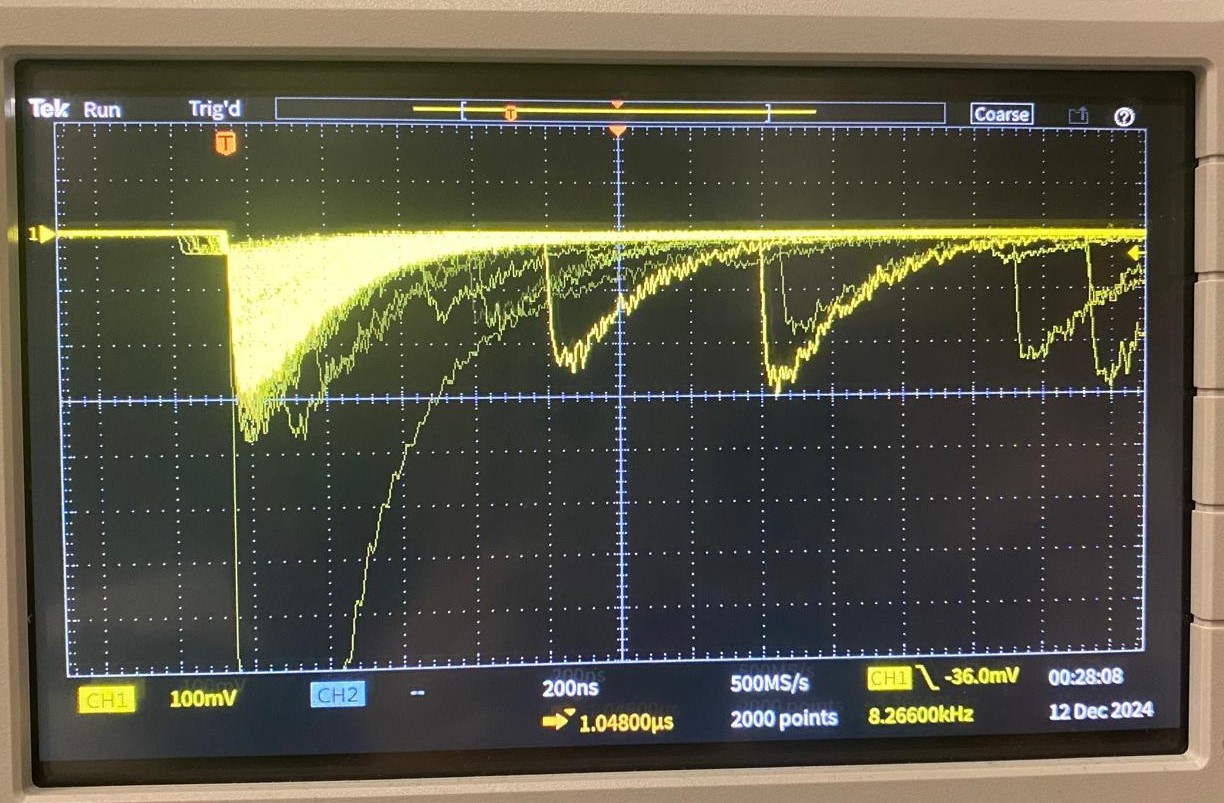
\includegraphics[height=0.23\linewidth]{signal.jpg}
    \quad\quad\quad
    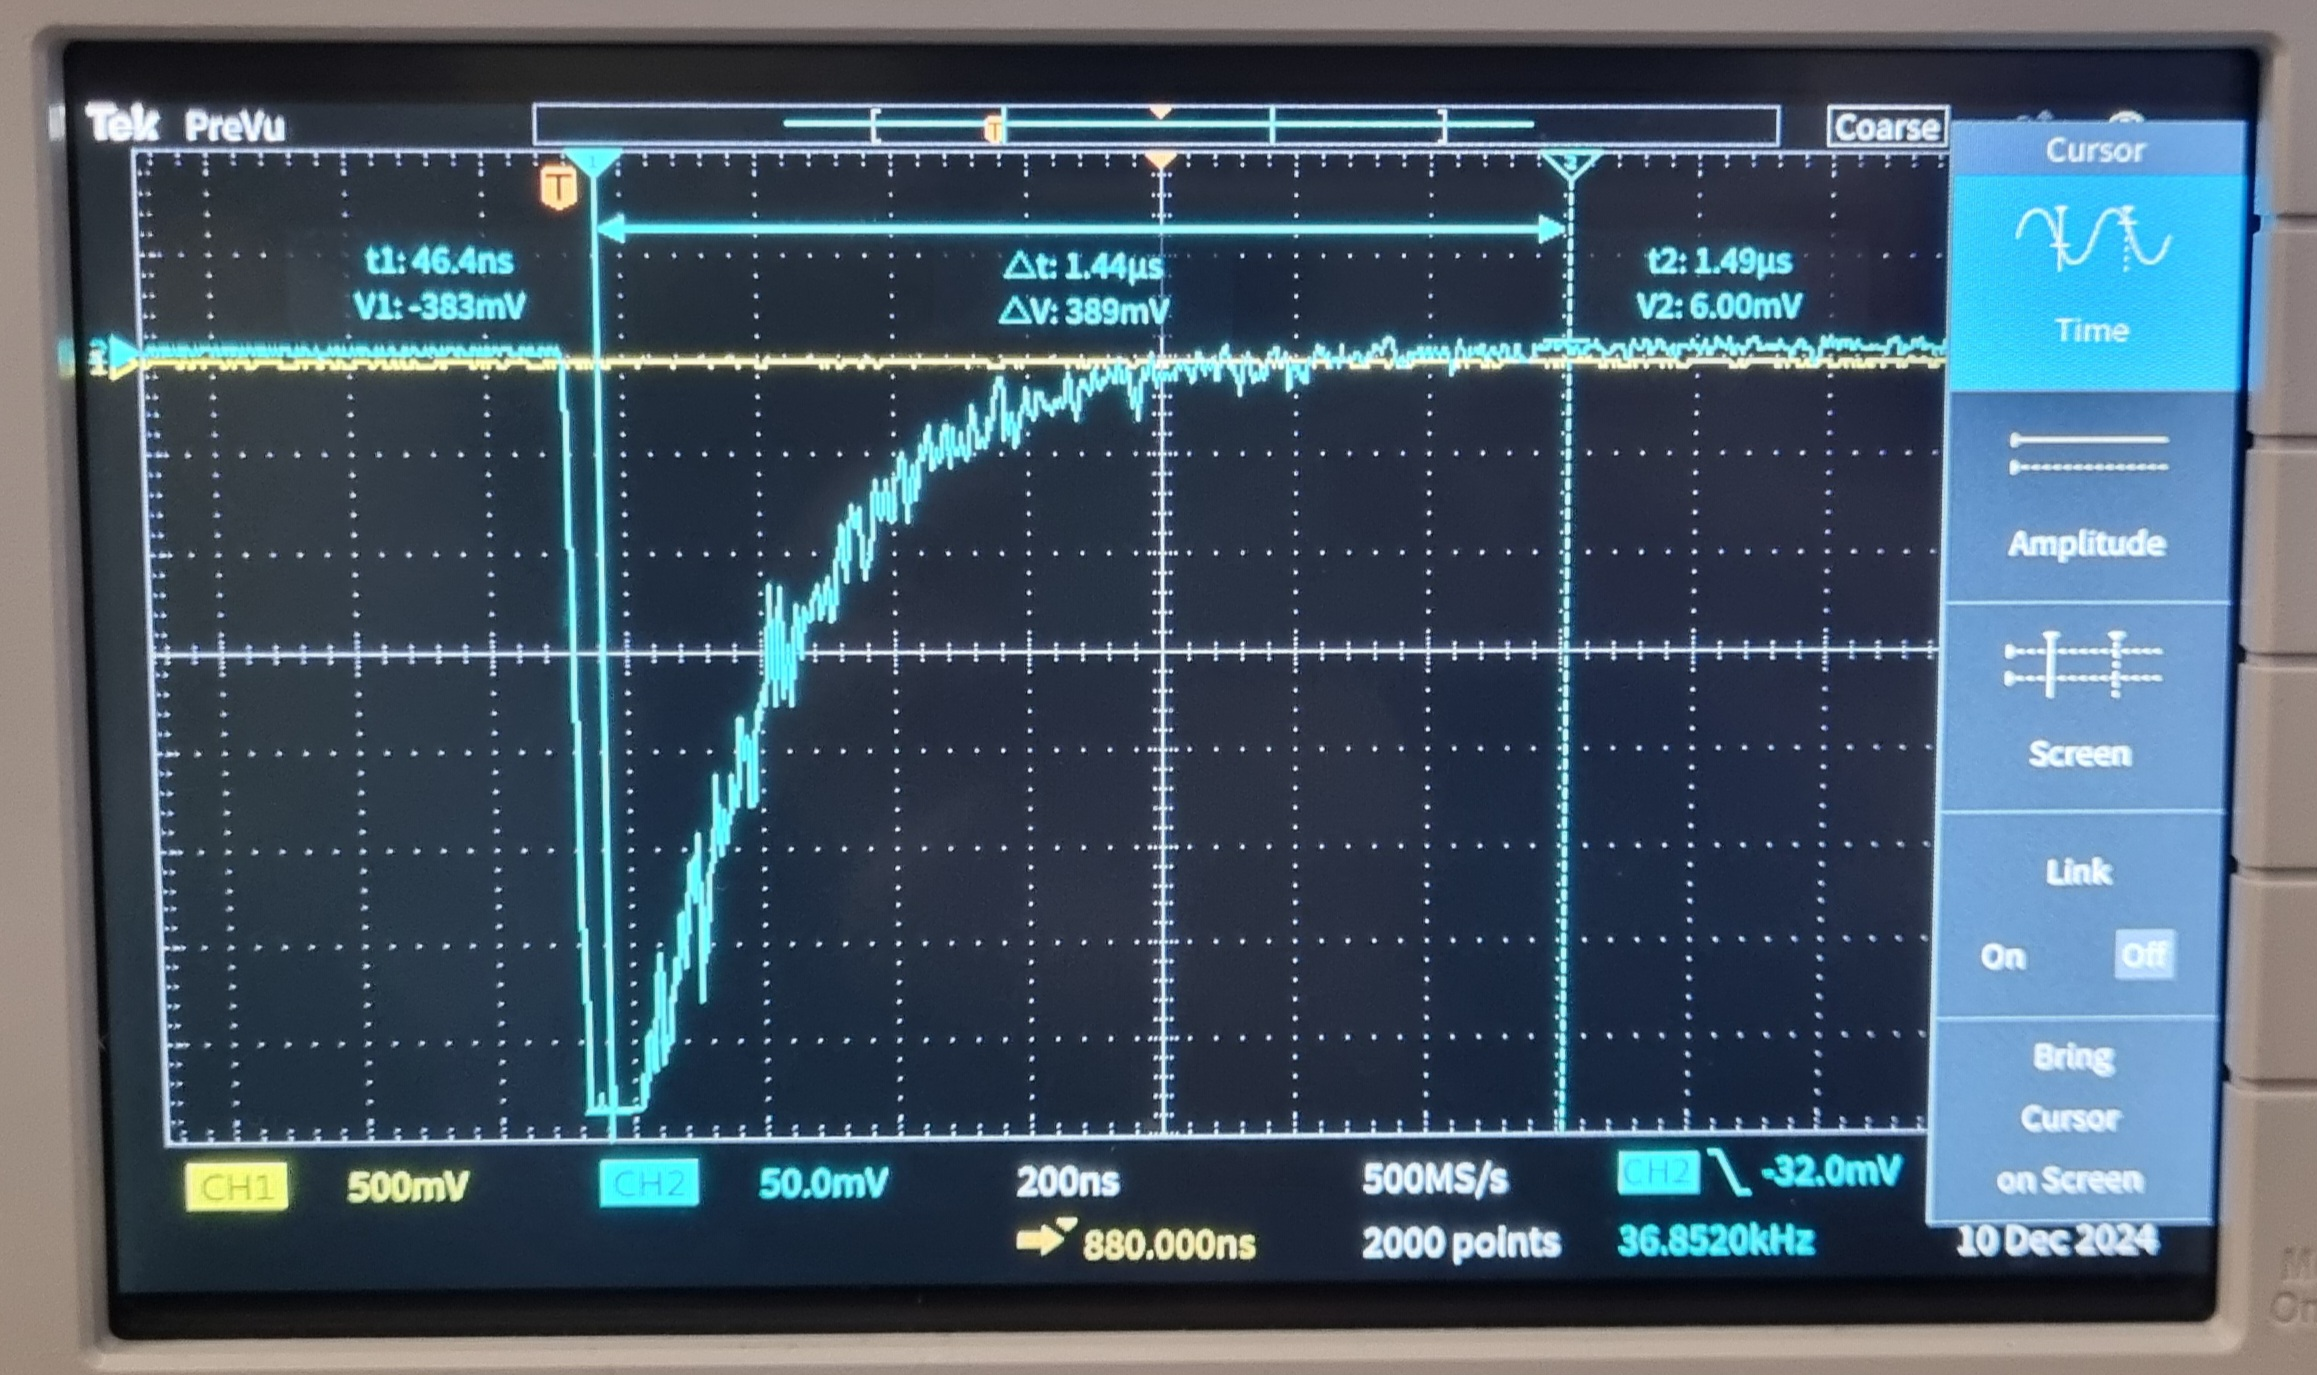
\includegraphics[height=0.23\linewidth]{signal1.jpg}
    \caption{Anode signals from the PMT of D\#1: on the right, a bunch of signals; on the left, a picture of just one of them.\protect\footnotemark} \label{fig:signals}
\end{figure}
\footnotetext{The characteristic values of the right picture are not correct, since the HV has been changed after taking the picture. The correct values are in Tab. \ref{tab:pmt_signals}.}

The next table (Tab. \ref{tab:pmt_signals}) shows the main values that describe the signals. The maximum amplitude and the noise level were measured by looking at all the signals together, whereas the time measurements were done with the cursors of the oscilloscope by taking only an example signal. Let us point out that, since no average was performed, then, 
% those signals are not obtained by means of more signals; therefore, 
especially for the amplitude measure, those values are just an example, so we present just an approximate value, obtained with the scale - \textit{division} - shown in brackets.
\begin{table}[H]
    \centering
    \captionsetup{width=.95\linewidth}
    \begin{tabular}{|l|ccccc|}
         \hline
         & $t_{\mathrm{fall}}\, \mathrm{(ns)}$ & $t_{\mathrm{rise}}\, \mathrm{(ns)}$ & $V_{\mathrm{max}}\, \mathrm{(mV)} $ & $V_{\mathrm{noise}}\, \mathrm{(mV)}$ & $V_{\mathrm{th}}\, \mathrm{(mV)}$\\
         \hline
         D\#1 & $\approx33.2(\mathrm{div}\,20)$ & $\approx670(\mathrm{div}\,100)$ & $\approx400(\mathrm{div}\,50)$ & $\approx15\!\divisionsymbol \!20(\mathrm{div}\,20)$ & $\approx 30$\\ 
         D\#2 & $\approx62.8(\mathrm{div}\,20)$& $\approx926(\mathrm{div}\,100)$  & $\approx364(\mathrm{div}\,100)$ & $\approx15\!\divisionsymbol \!20(\mathrm{div}\,20)$ & $\approx 30$\\
        \hline         
    \end{tabular}
    \caption{Example of the characteristic values of an anode signal from the PMT of D\#1 and D\#2: falling time, rising time, maximum peak height, noise level and CFD threshold estimation. The values in the brackets are the division scale.} 
    \label{tab:pmt_signals}
\end{table}

Each PMT output was used as the input of a CFD. The CFDs thresholds (Tab. \ref{tab:pmt_signals}) were put at a minimum level, considering the noise value. %why is that high? 
The CFDs outputs were fed to a coincidence unit, whose output, in turn, was used as the trigger of the digitizer.
% For the analysis related to the geometry of the experiment, Sect. \ref{position} and \ref{angular}, and to the efficiency of the detector, Sect. \ref{sect. efficiency}, the trigger of the digitizer was connected to the output of the Logic Unit. 
The modality of the coincidence could be varied in "OR" or "AND" mode. A picture of the CFDs outputs is provided in Fig. \ref{fig:coincidence}: the widths of the signals and the delay between them (Tab. \ref{tab:widths}) are such to create the coincidence.
\begin{figure}[htp]
\centering
\hfill
\begin{minipage}[b]{.4\columnwidth}
  \centering
  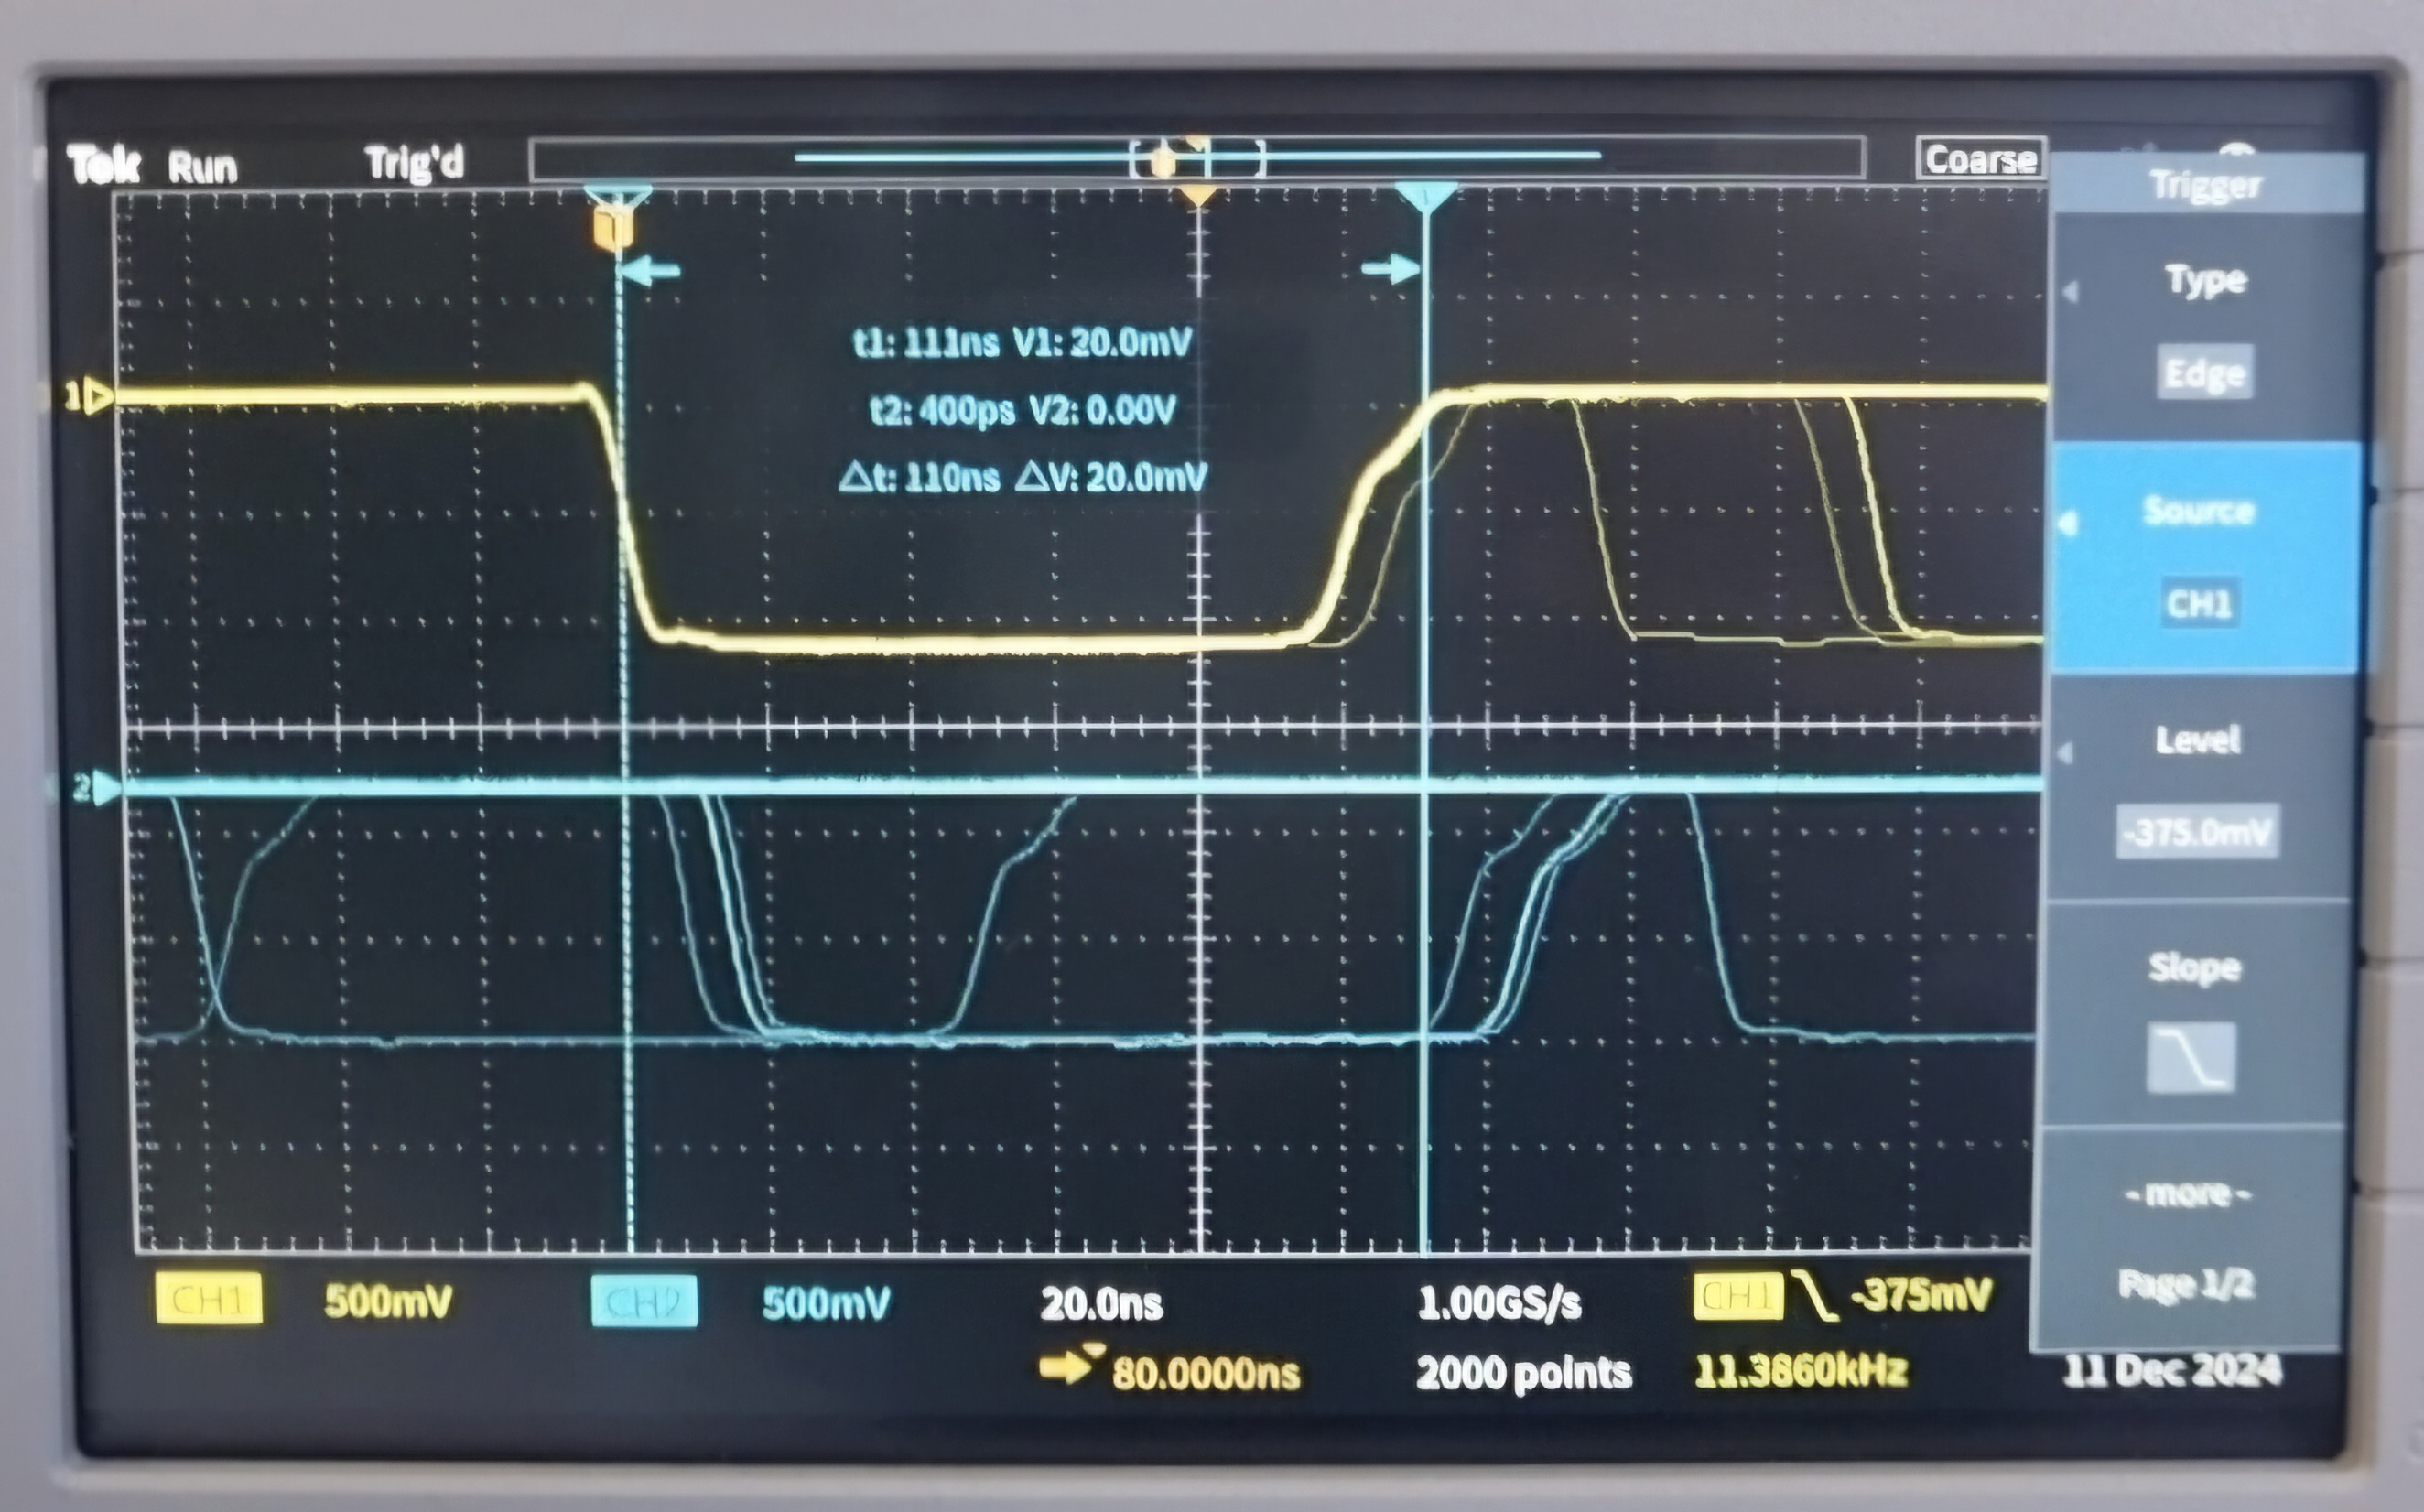
\includegraphics[width=1.0\linewidth]{signal2.jpg}
  \caption{Output signals from CFDs: D\#1 is on Ch1 of the oscilloscope, whereas delayed D\#2 on Ch2. The two signals, whose widths are of  $\approx100\,\mathrm{ns}$, have an overlapping region.}\label{fig:coincidence}
\end{minipage}\hfill
\begin{minipage}[b]{.4\columnwidth}
  \centering
  \begin{tabular}{|c|c|c|}
        \hline
        &Width (ns) & Delay (ns)\\
        \hline
         D\#1& $\approx98.8 (\mathrm{div}\,20)$ & \multirow{2}*{$\approx15$}\\
         D\#2& $\approx110 (\mathrm{div}\,20)$& \\
        \hline
    \end{tabular}
  \captionof{table}{Widths of the CFDs output signals and relative external delay. The values in the brackets are the division scale.}
  \label{tab:widths}
\end{minipage}\hspace*{\fill}
\end{figure}

% \begin{figure}[H]
%     \centering
%     \captionsetup{width=.87\linewidth}
%     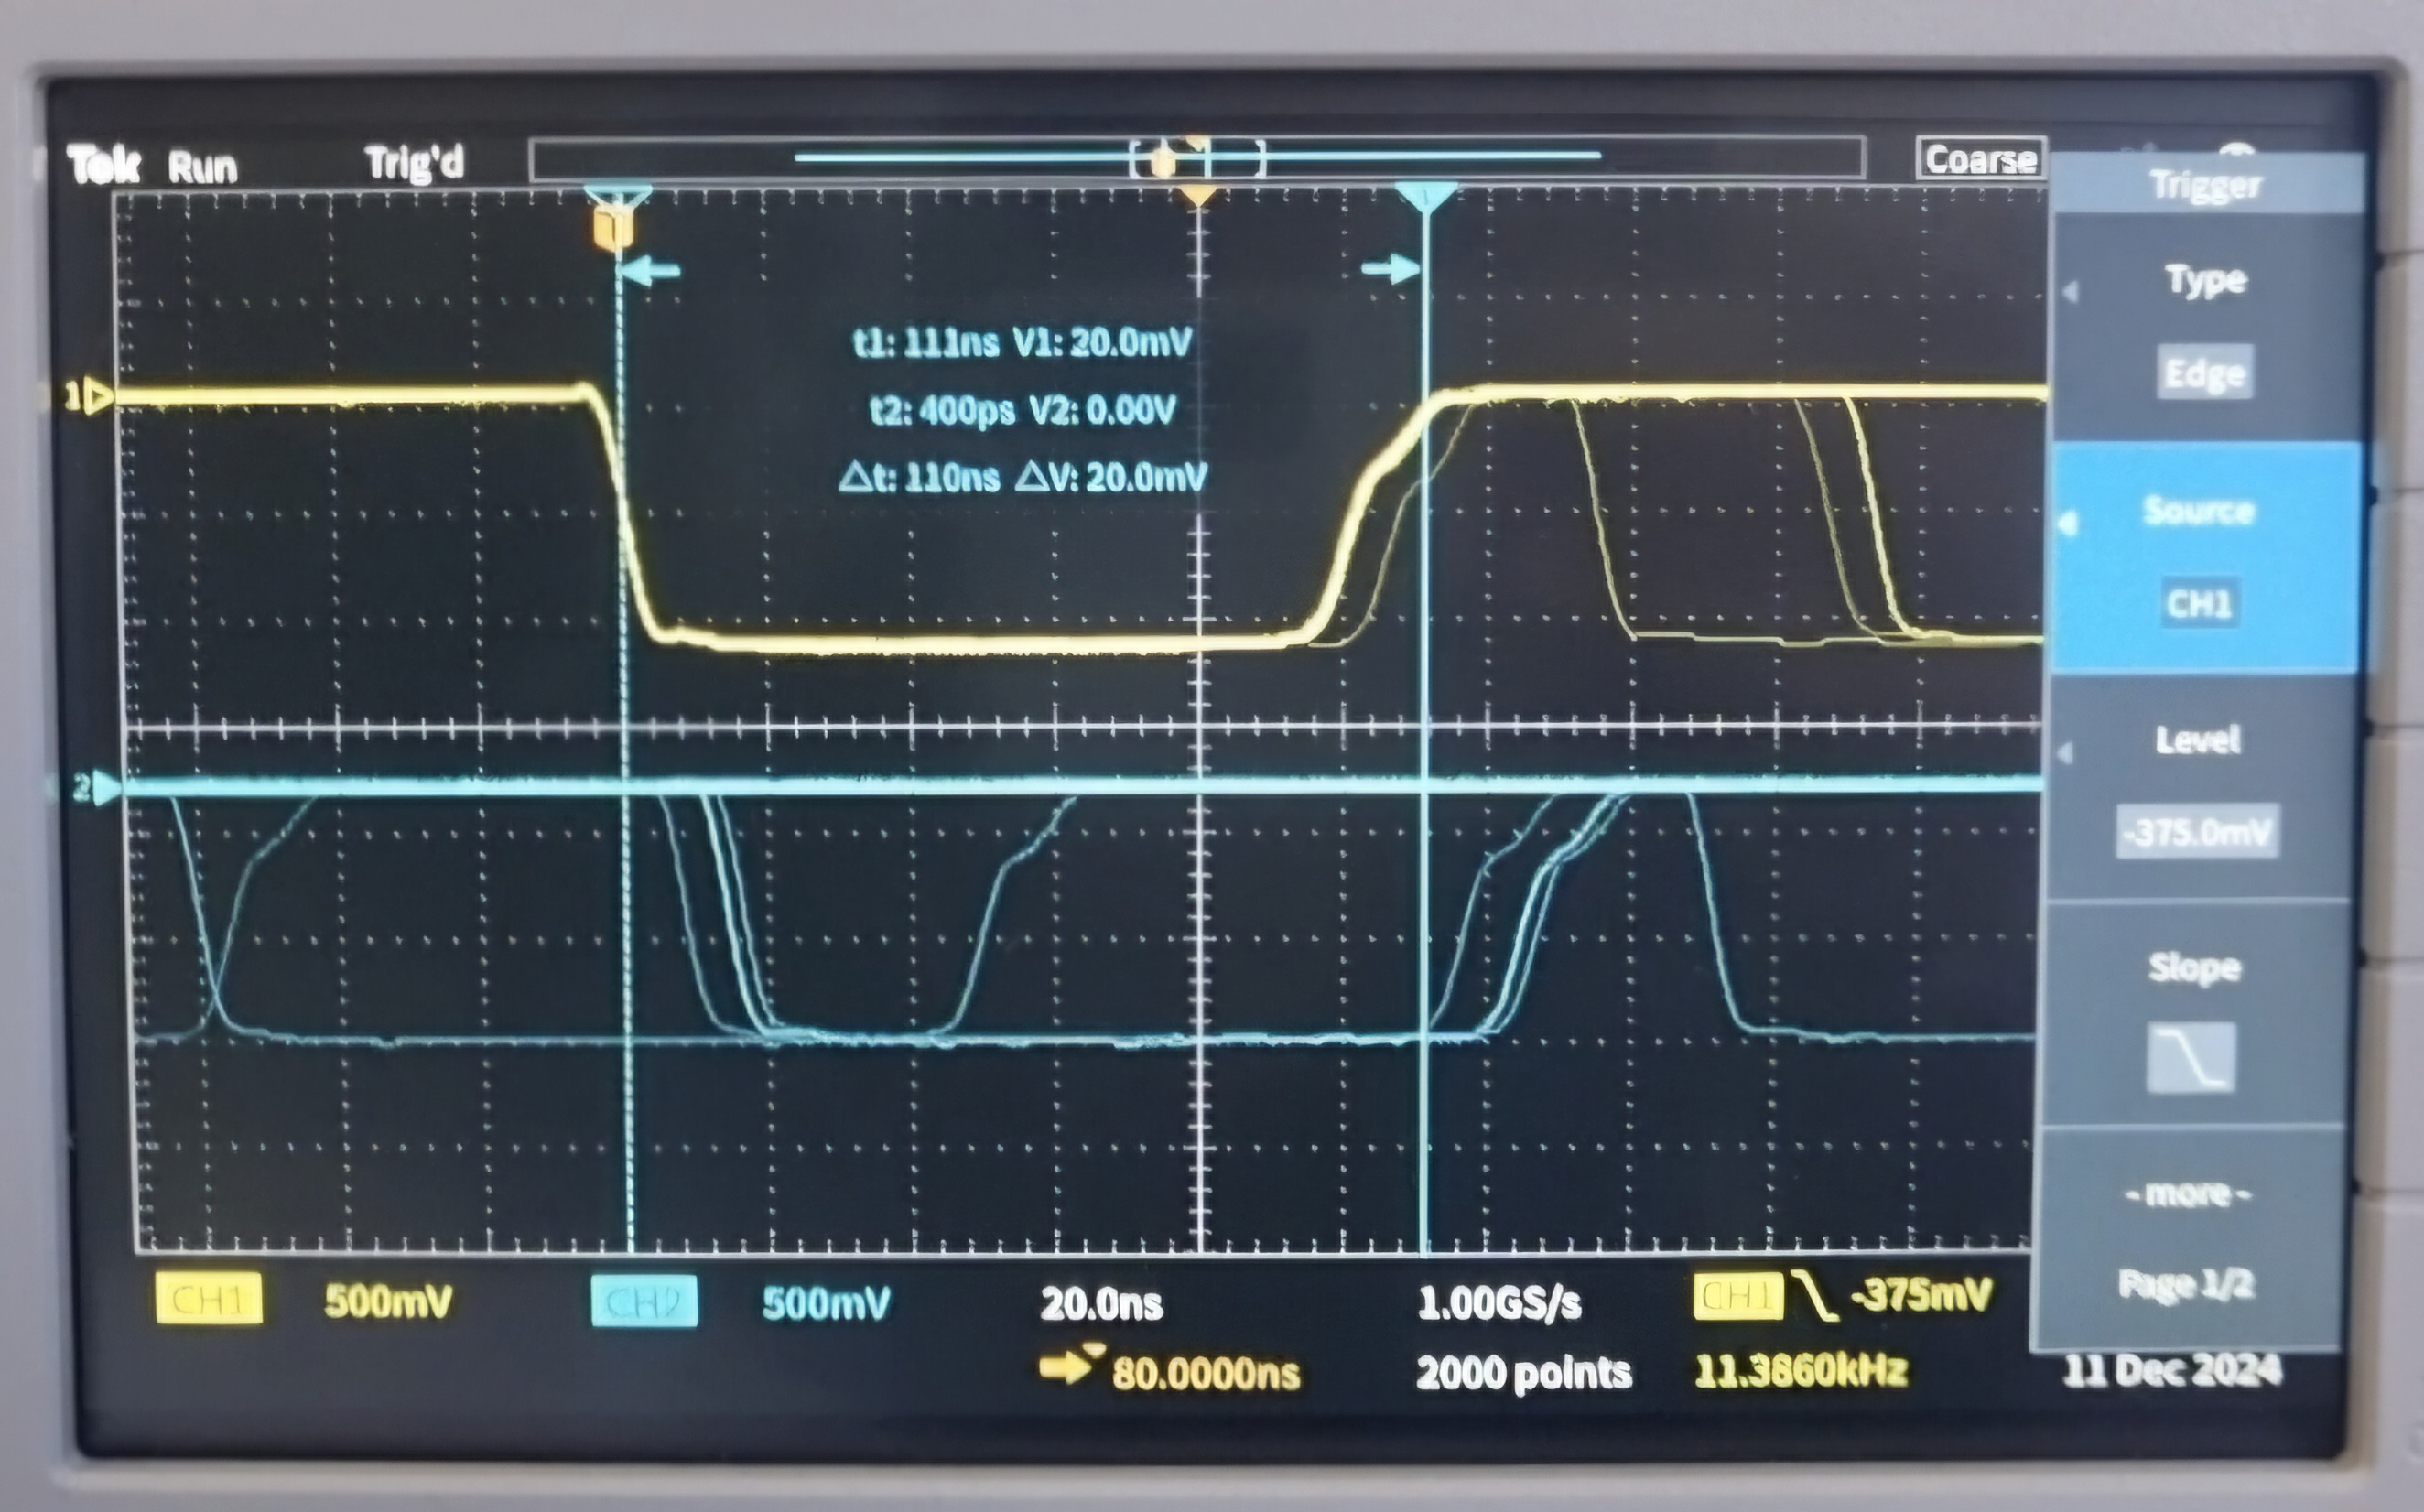
\includegraphics[width=0.40\linewidth]{signal2.jpg}
%     \caption{Outputs from CFDs: D\#1 is on Ch1 of the oscilloscope, whereas delayed D\#2 on Ch2. The two signals, whose widths are of  $\approx100\,\mathrm{ns}$, have an overlapping region.}
%     \label{fig:coincidence}
% \end{figure}
% \vspace{-0.3cm}
% \begin{table}[H]
%     \centering
%     \begin{tabular}{|c|c|c|}
%         \hline
%         &Width (ns) & Relative delay (ns)\\
%         \hline
%          D\#1& $\approx98.8 (\mathrm{s.}20)$ & \multirow{2}*{$\approx15$}\\
%          D\#2& $\approx110 (\mathrm{s.}20)$& \\
%         \hline
%     \end{tabular}
%     \caption{Widths of the signals from the CFDs and delay\protect\footnotemark}
%     \label{tab:widths}
% \end{table}
% \footnotetext{The values in the brackets are the division scale.}
% \vspace{-0.3cm}

\subsubsection{Energy calibration} \label{sect:energy calibration}
Another fundamental aspect of the preliminary analysis is the energy calibration of the detectors. To do so, two channel spectra (Fig. \ref{fig:spectra_energy cal}, upper x-axes), one for each detector, were acquired for $180\,\mathrm{s}$ each, triggering on D\#1 and D\#2 respectively. %D#2 was at 30cm
\begin{figure}[H] 
    \centering
    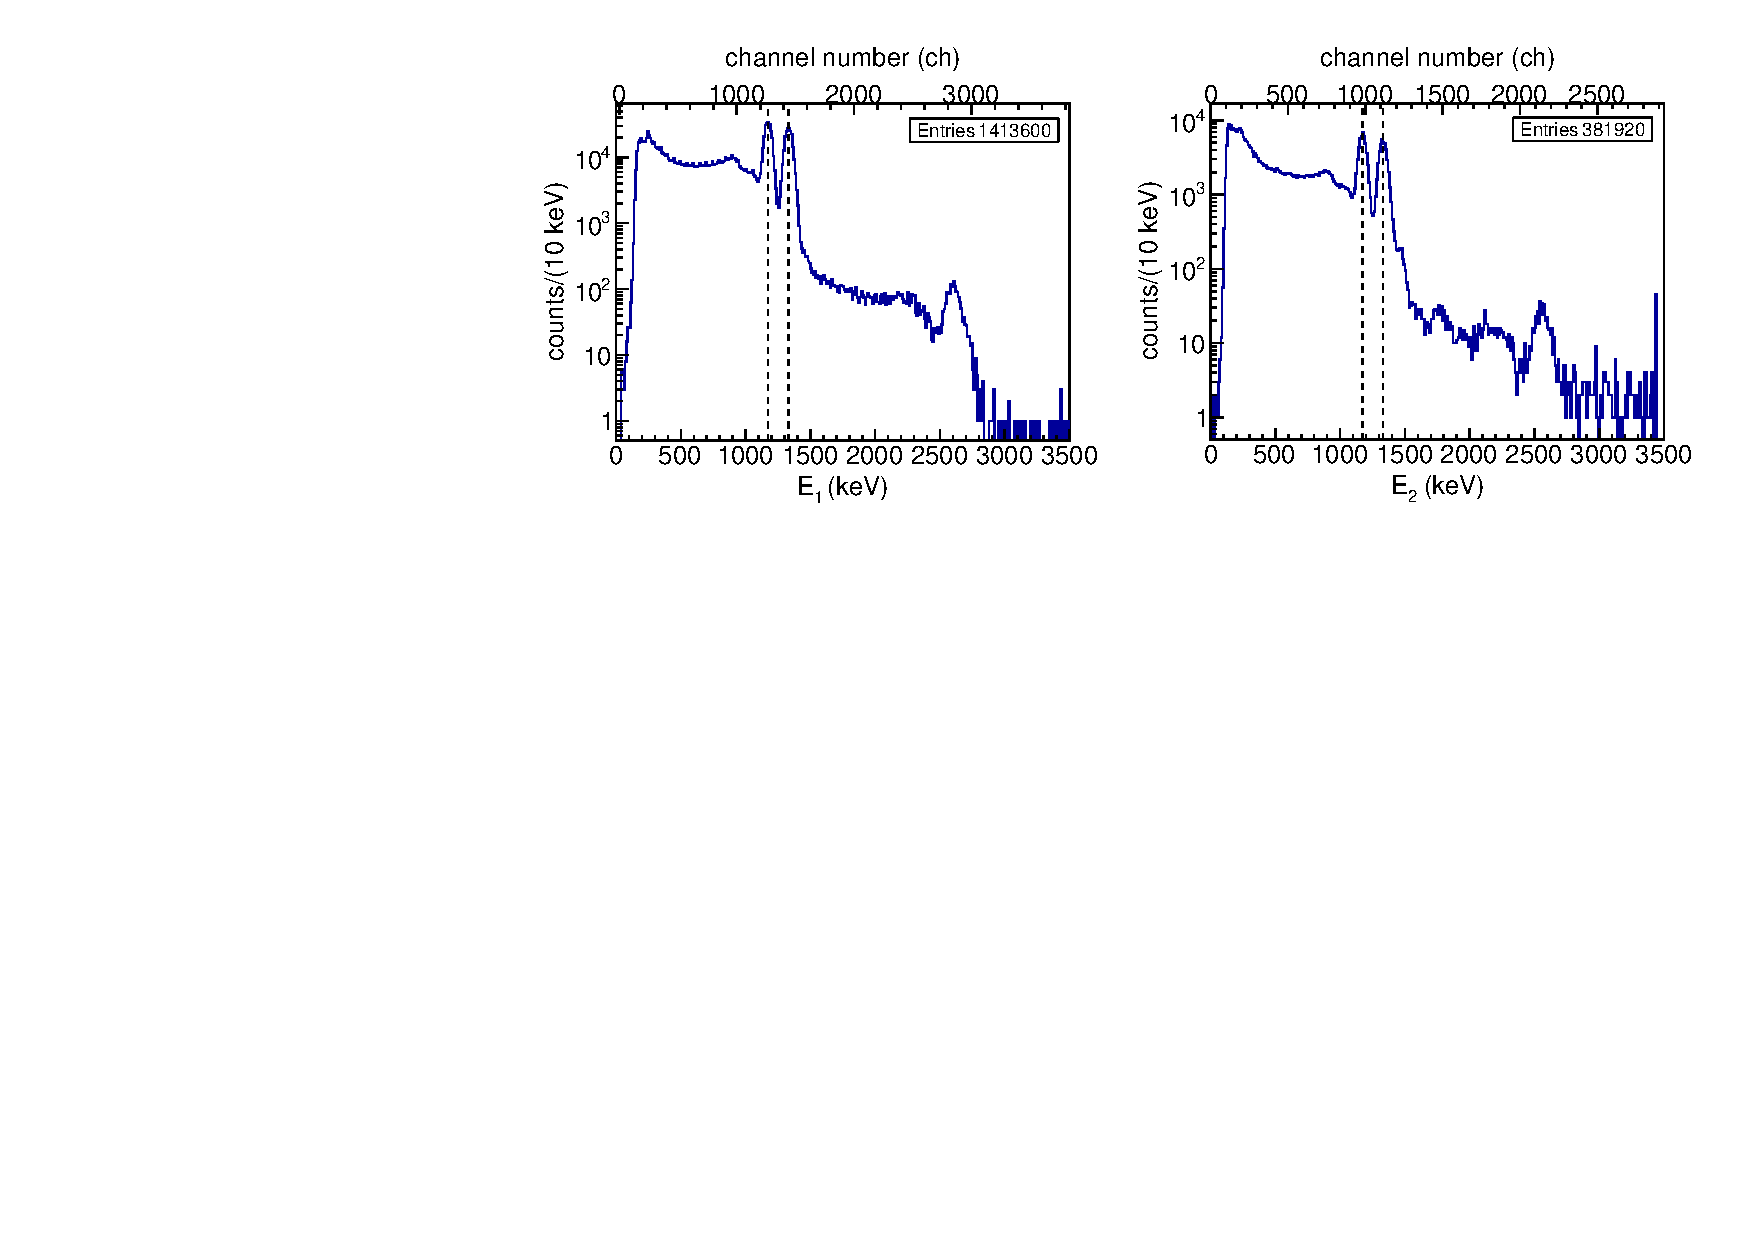
\includegraphics[width=\linewidth]{Energy_cal/cal_histos.pdf}
    \caption{Spectra for energy calibration, triggered by D\#1 (left) and D\#2 (right). The dashed lines highlight the peaks used for the calibration. On the lower x-axes it is possible to see the calibrated scale. The sum peak is not perfectly calibrated.} 
    \label{fig:spectra_energy cal}
\end{figure}

The two peaks of the emitted photons will be used to obtain a two-point linear fit. It would be useful to have more points %are required in order 
to gain a better calibration at lower energies, which is helpful to study properly the background. 
In particular, for low energies a source of \ce{^241}Am may be used to have a peak at $59\,\mathrm{keV}$. However, with the set HV values, this peak was not visible for none of the detectors.

Tab. \ref{tab:cal_centroids} shows the values of the centroids $C_1$ and $C_2$ for D\#1 and D\#2 respectively, obtained with Gaussian fits on the peaks. The interpolation (Fig. \ref{fig:calibration}) gives the results shown in Tab. \ref{tab:cal_fit}.

\begin{table}[H]
    \centering
    \begin{tabular}{|c|ccc|}
      \hline
       Photon&Energy $\mathrm{(keV)}$ & $C_1\,\mathrm{(ch)}$& $C_2\,\mathrm{(ch)}$\\
      \hline
      $\gamma_a$& $1173$ & $1050.18 \pm 0.06$ & $1399.5 \pm 0.2$\\ %l'errore su D2 ha un'ordine di grandezza in più, questo potrebbe essere dovuto ai meno eventi presenti dal momento che il detector era più lontano
       $\gamma_b$&$1332$ & $1196.45 \pm 0.07$ & $1589.4 \pm 0.2$\\
      \hline
    \end{tabular}
    \caption{Energy of the peaks (keV) and centroids (ADC channels) for D\#1 and D\#2}
    \label{tab:cal_centroids}
\end{table}
\vspace{-0.5cm}

\begin{figure}[H]
    \centering
    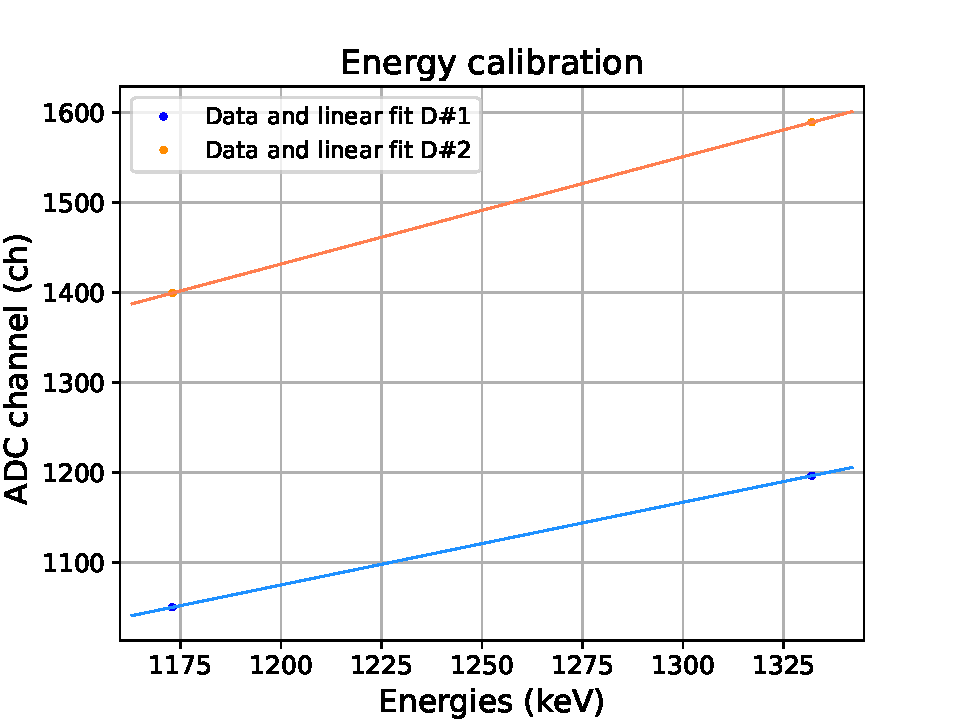
\includegraphics[width=0.45\linewidth]{Energy_cal/calibration.pdf}
    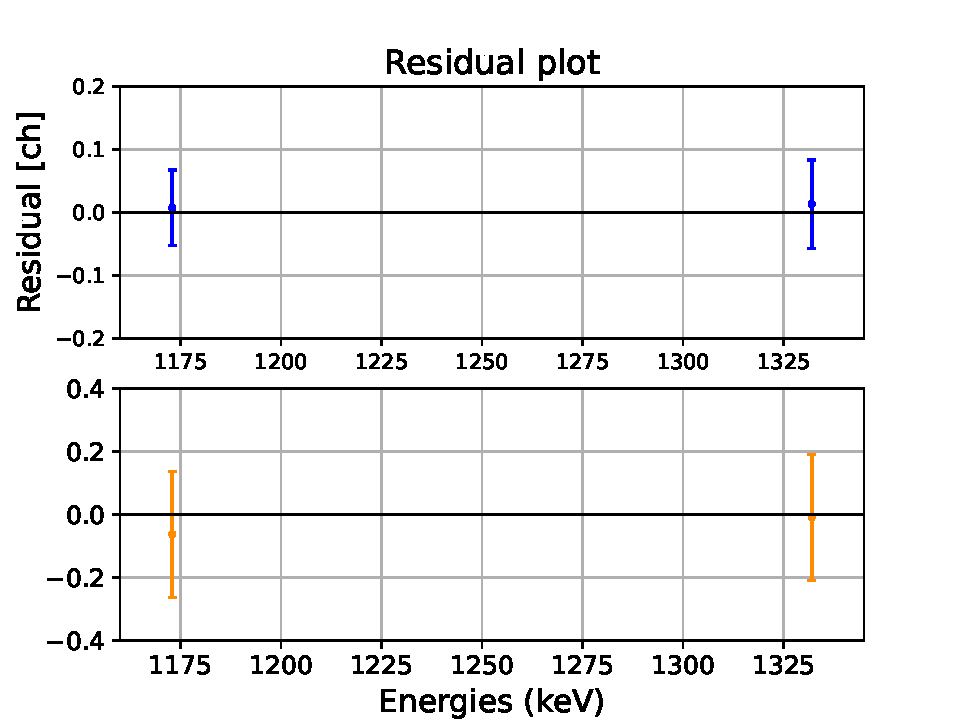
\includegraphics[width=0.45\linewidth]{Energy_cal/cal_res.pdf}
    \caption{Linear fit and residual plots for energy  calibration (see Tab. \ref{tab:cal_centroids})} 
    \label{fig:calibration}
\end{figure}

\begin{table}[H]
    \centering
    \begin{tabular}{|l|cc|}
    \hline
     D\#1 & $m_1=0.9199\pm0.0006\,\frac{\mathrm{ch}}{\mathrm{keV}}$ &  $q_1=-28.9\pm0.7 \,\mathrm{ch}$\\
     D\#2 & $m_2=1.194\pm0.002\,\frac{\mathrm{ch}}{\mathrm{keV}}$ & $q_2=-1\pm2\,\mathrm{ch}$\\ 
    \hline        
    \end{tabular}
    \caption{Fit parameters for linear fit $C_i=m_i\cdot E+q_i$, with $i=1,2$ the detector number.}
    \label{tab:cal_fit}
\end{table}

Now it is possible to use these parameters to calibrate the spectra, which are shown on the lower x-axis of Fig. \ref{fig:spectra_energy cal}, and to calculate the resolution of the peaks (Tab. \ref{tab:resolution}), for both detectors, as 
$$R\,[\mathrm{\tfrac{keV}{keV}}]=\dfrac{\mathrm{FWHM}}{C}=2.35\cdot\dfrac{\mathrm{\sigma_C}}{C}$$
\begin{table}[H]
    \centering
    \begin{tabular}{|c|ccc|}
         \hline
          & $C\,\mathrm{(keV)}$ & $\mathrm{FWHM\,(keV)}$ & $R\,(\%)$ \\
         \hline
          \multirow{2}*{D\#1} &$1173\pm1$ & $65.9\pm0.1$ & $5.61\pm0.03$ \\
                              &$1332\pm1$ & $68.9\pm0.2$ & $5.17\pm0.03$\\
        \hline
          \multirow{2}*{D\#2} &$1173\pm3$ & $69.9\pm0.5$ & $5.86\pm0.09$\\
                              &$1332\pm3$ & $70.9\pm0.5$ & $5.32\pm0.08$\\
         \hline
    \end{tabular}
    \caption{Resolutions of the calibrated spectra}
    \label{tab:resolution}
\end{table}



\subsubsection{Position of the source} \label{position}
%I'm going to fix and complete the text according to your suggestions
The aim of this section is to check if the source was correctly placed at the point $O$, where the detector axes intersect, which defines the rotation axis of D\#2. 
This can be done by checking if the singles count rate recorded by D\#2 varies significantly with the angle between detector axes. 
In fact, miscentering of the source will make the source - D\#2 separation depend on the angle, thus introducing a merely geometrical angular dependence of the count rate.

Let $\theta$ be the angular displacement of D\#2 with respect to the axis that connects $O$ to D\#1, measured anticlockwise. 
The nominal source-detectors distances were approximately $d_1\approx12.5\text{ cm}$, $d_2\approx31.5\text{ cm}$. %Detector\#2 was set $(31.5\pm ...)$ cm far from its rotation axis.\footnote{From this Section on, this distance will be unchanged.} 
Using the "OR" of the detectors as the trigger signal, a 5-minute acquisition was recorded for each of six different nominal $\theta$ angles, shown in Tab. \ref{tab:source position} without errors. The number of recorded events  $N_\mathrm{events}$ is shown in the same Table and plotted in Fig. \ref{fig:source position}. The uncertainties were calculated as the statistical error of a Poisson distribution, i.e. $\sigma=\sqrt{N_\mathrm{events}}$.
\begin{table}[H]
\parbox{.45\linewidth}{
 \centering 
 \captionsetup{width=.8\linewidth}
    \begin{tabular}{|c|c|}
    \hline
        $\theta$ & $N_\mathrm{events}$ ($\times10^6$) \\
        \hline
        $90^\circ$ & $2.971\pm0.002$\\
        $110^\circ$ & $2.966\pm0.002$\\
        $130^\circ$ & $2.966\pm0.002$\\
        $140^\circ$ & $2.962\pm0.002$\\
        $160^\circ$ & $2.958\pm0.002$\\
        $180^\circ$ & $2.957\pm0.002$\\
        \hline
    \end{tabular}
    \caption{Total number $N_\mathrm{events}$ of recorded events in the "OR" acquisition with relative angular displacement $\theta$}
    \label{tab:source position}}
     \hspace{-4 cm}
\parbox{.55\linewidth}{
\centering
\begin{figure}[H]
    \centering
    \captionsetup{width=.5\linewidth}
    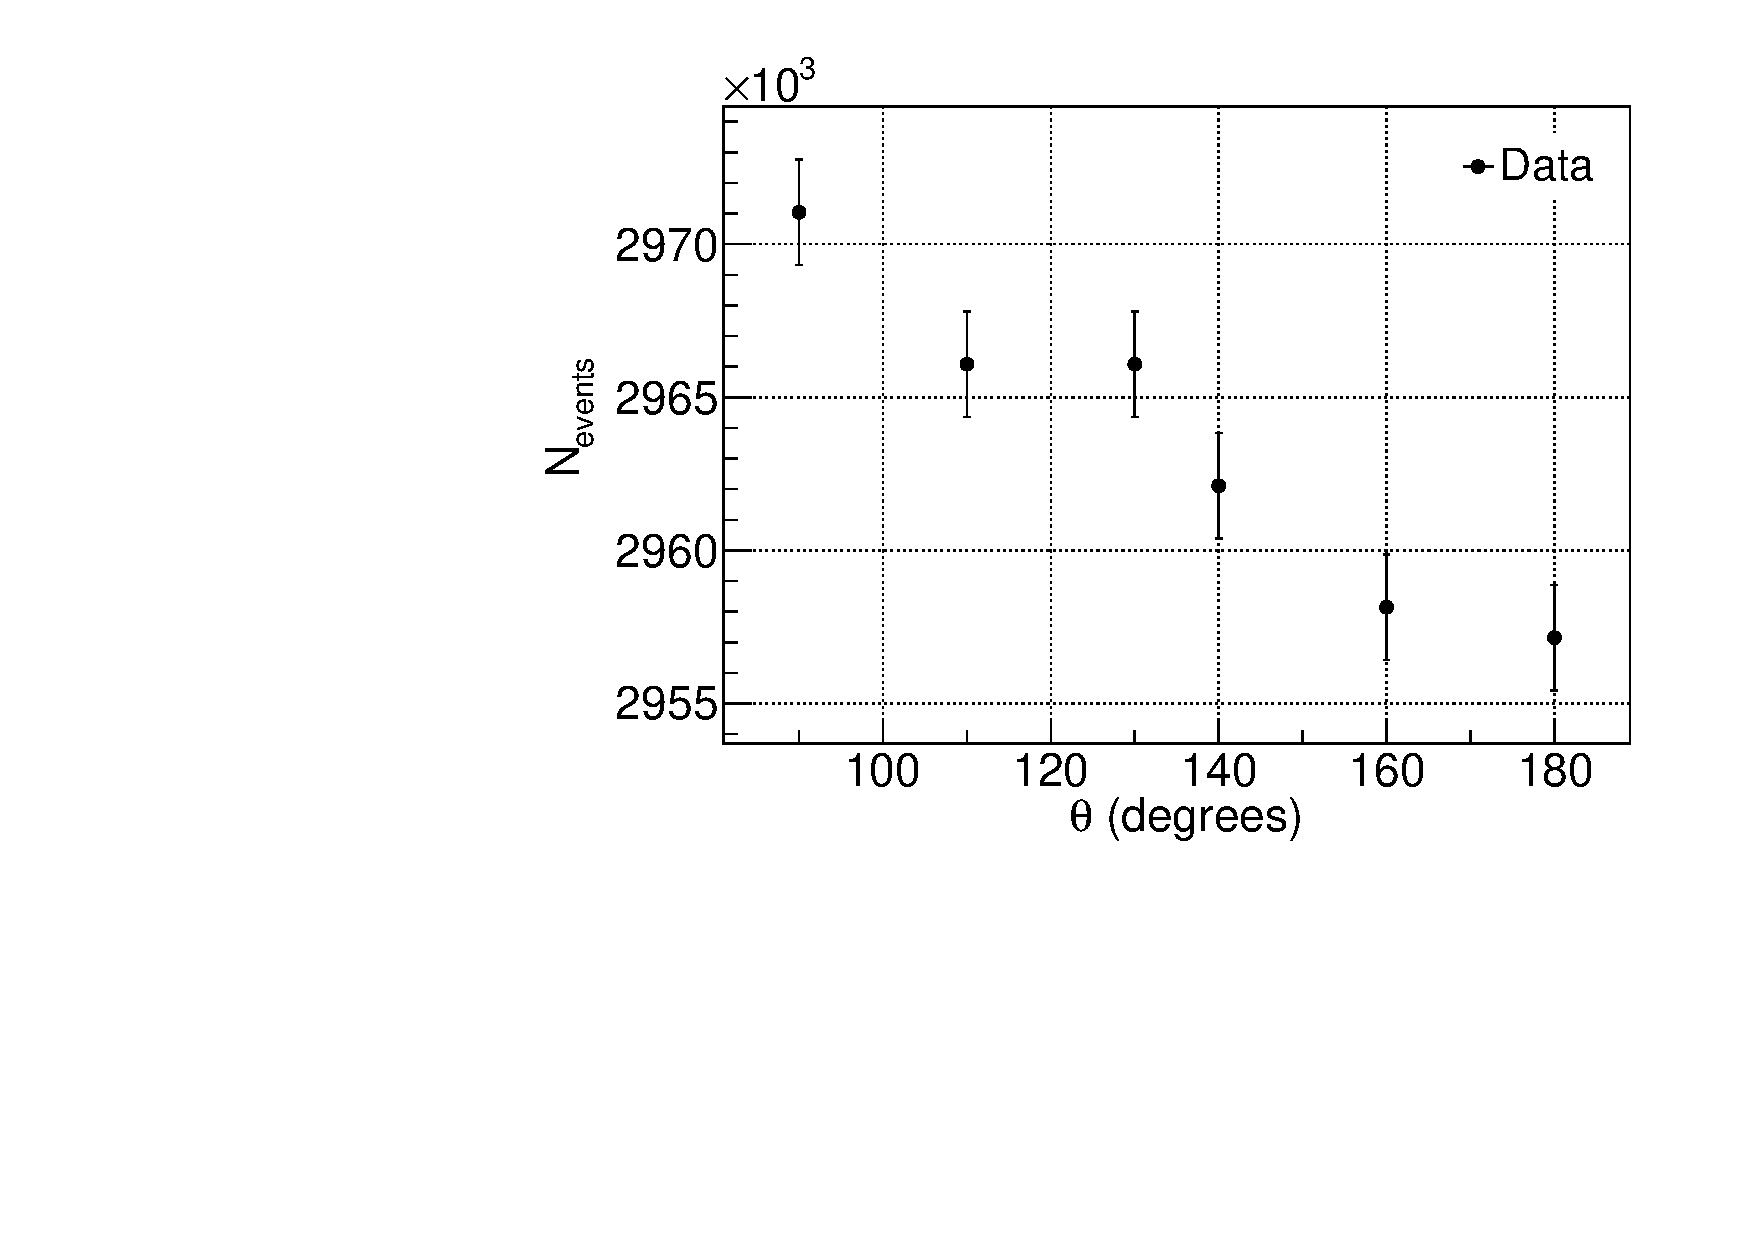
\includegraphics[width=0.5\linewidth]{geometry/geom5.pdf}
    \caption{Total number of recorded events in the "OR" acquisition with relative angular displacement $\theta$}% (see Tab. \ref{tab:source position})}
    \label{fig:source position}
\end{figure}}
\end{table}

\vspace{-0.5cm}

These experimental data show a statistically relevant decreasing trend as $\theta$ is increased, thus suggesting that the source was placed closer to the $90^\circ$ D\#2 configuration than to the $180^\circ$ one. The total reduction between $90^\circ$ and $180^\circ$ is $0.5\%$.

This geometrical angular dependence may affect the accuracy of the measurement of the angular correlation, which is the topic of the next Section. 
At first order, the coincidence counts used to measure the correlation function could be corrected by normalizing them with respect to the singles count rate recorded by D\#2. However, since the source was moved during the time between the assessment of the source position and the measurement of the angular correlation, this correction cannot be made and only an error estimate will be performed.


\subsection{Study of the angular correlation function} \label{sect: angular}
% \textcolor{blue}{Relative yield of $\gamma_2$ about the $\theta$ direction given that $\gamma_1$ is emitted in the $0^\circ$ direction:}
The angular correlation function $w(\theta)$ for a $\gamma-\gamma$ cascade can be written as
\begin{equation}\label{eq:w(theta)}
        w(\theta)\equiv\frac{N(\theta)}{N(\pi/2)}=1+c_2'\cos^2(\theta)+c_4'\cos^4(\theta)
\end{equation}
where $N(\theta)$ is the number of coincidence counts such that the first $\gamma$-ray is detected about the $\theta$ direction and the second $\gamma$-ray is emitted in the $0^\circ$ direction. 
Due to finite instrumental angular resolution, the factors $c_2'$ and $c_4'$ are expected to be lower than the theoretical ones, which are $c_2=0.125$ and $c_4=0.042$.
% \textcolor{blue}{The directional correlation between the two $\gamma$-rays in cascade may be measured by recording the first $\gamma$-ray in one of the detectors and the second $\gamma$-ray in the other and measuring the number of coincidences at different angles.}

In order to evaluate this function, a 35-minute acquisition was performed in coincidence (“AND” signal as trigger) at each of six different angles $\theta$, shown in Tab. \ref{tab:angular corr function}. 
Figure \ref{fig:angular correlation scatter plot theta=0} shows the correlation between the calibrated energies $E_1$ and $E_2$ deposited in D\#1 and D\#2, respectively, for the case $\theta=0^\circ$.
\vspace{-0.4cm}

% Per scommentare basta fare Ctrl^ù
% \begin{table}[H]
%  \centering
%     \begin{tabular}{|c|cc|}
%     \hline
%         $\theta$ & $N_{ab}(\theta)\times10^3$  &$w(\theta)$\\
%         \hline
%         $90^\circ$ & $1.83\pm0.04$ & $1.00\pm0.03$\\
%         $110^\circ$ & $1.76\pm0.04$& $0.96\pm0.03$\\
%         $130^\circ$ & $1.86\pm0.04$&$1.01\pm0.03$\\
%         $140^\circ$ & $1.96\pm0.04$ & $1.07\pm0.03$\\
%         $160^\circ$ & $2.00\pm0.04$&$1.09\pm0.03$\\
%         $180^\circ$ & $1.87\pm0.04$ &$1.02\pm0.03$\\
%         \hline
%     \end{tabular}
%     \caption{Number of selected events and angular correlation function calculated with fit results}
%     \label{tab:angular corr function}
% \end{table}

\begin{figure}[H]
    \centering
    \captionsetup{width=\linewidth}
    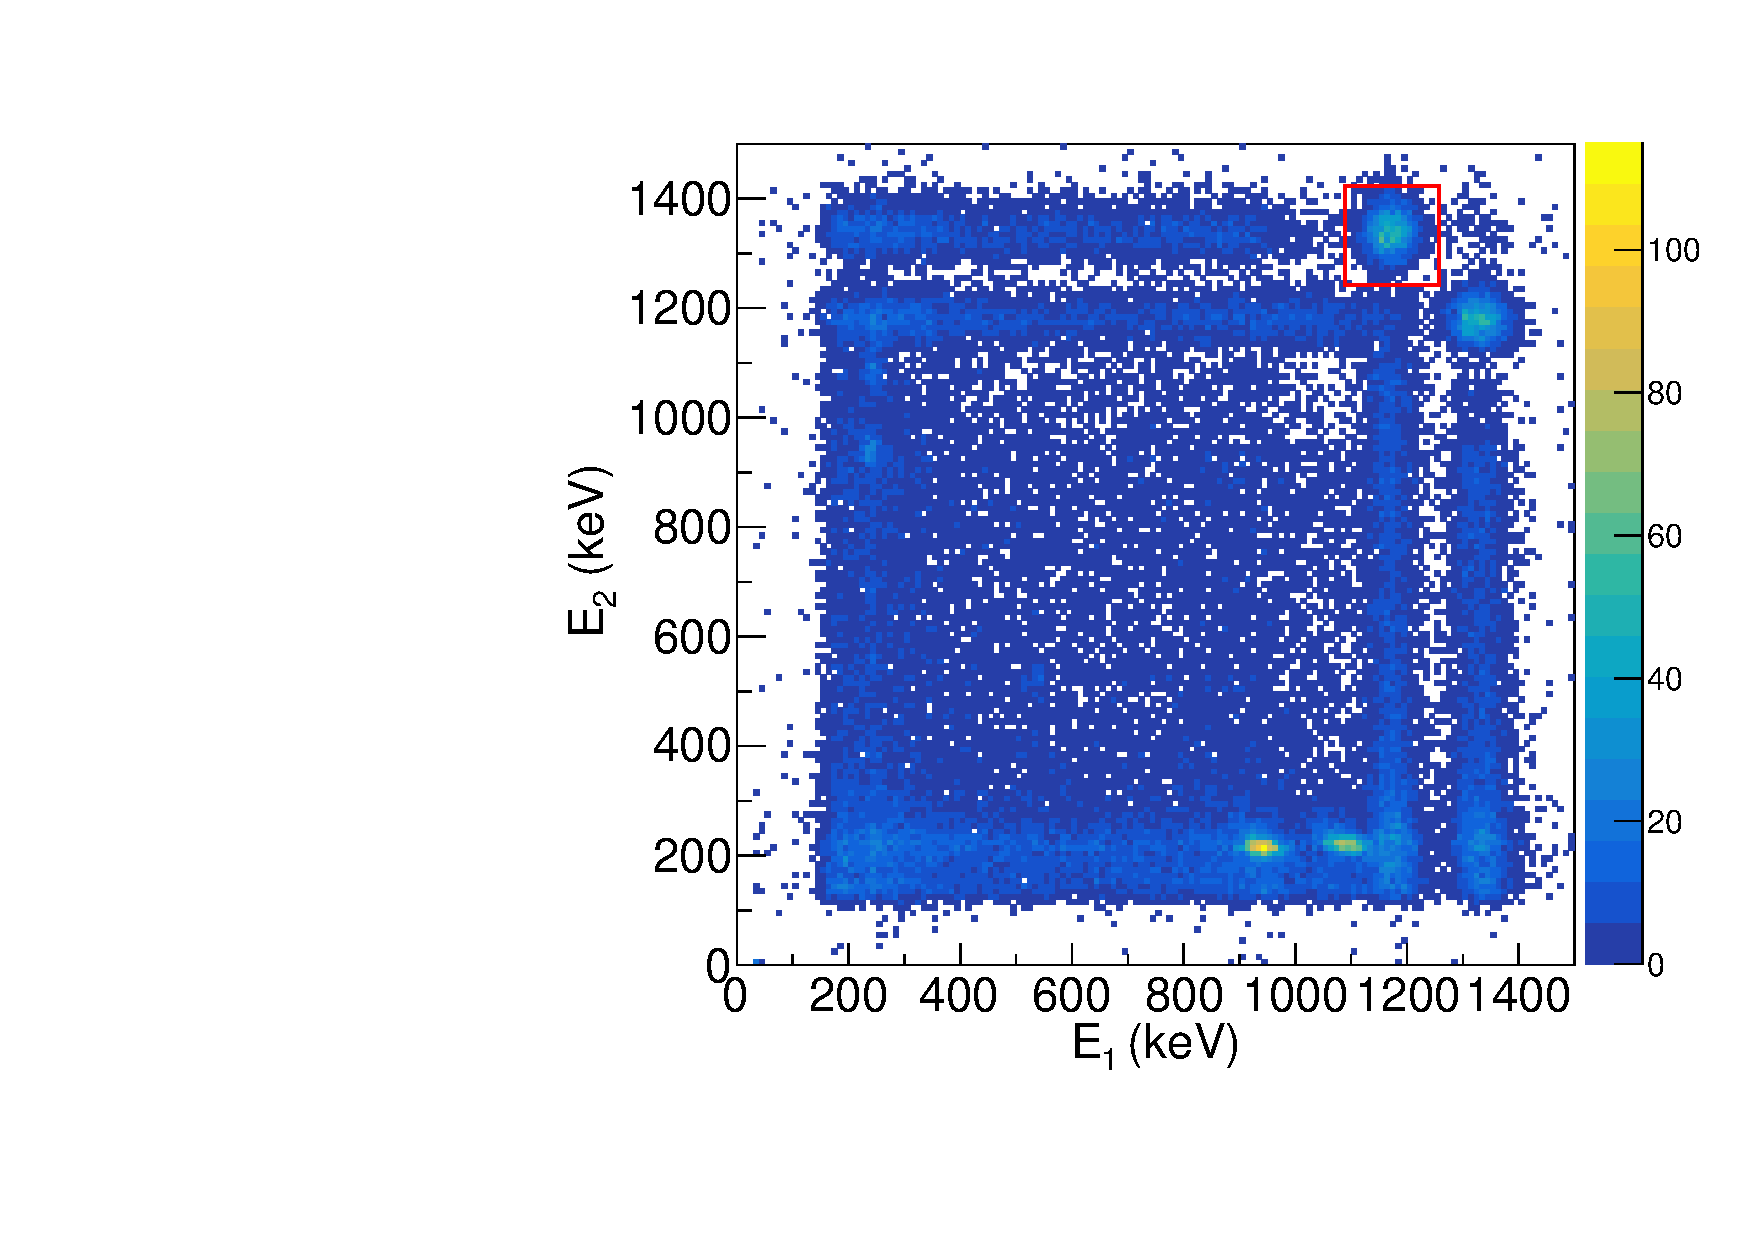
\includegraphics[width=0.45\linewidth]{Angular_Corr/Scatter_AngCorr3.pdf}
    \caption{Correlation between the energy $E_1$ released in D\#1 and the energy $E_2$ released in coincidence in D\#2 placed at $\theta=0^\circ$. The red rectangle shows the selection of events for the angular correlation measurement.}
    \label{fig:angular correlation scatter plot theta=0}
\end{figure}

The peaks centred at $(E_1,E_2)\!=\!(1173\;\mathrm{keV}, 1332\;\mathrm{keV})$ and $(E_1,E_2)\!=\!(1332\;\mathrm{keV}, 1173\;\mathrm{keV})$ correspond to the coincidence full energy absorption of both $\gamma$-rays, one in D\#1 and the other in D\#2. In particular, the $(1173\;\mathrm{keV}, 1332\;\mathrm{keV})$ peak is populated by events in which the first photon is detected by D\#1 and the second photon by D\#2; thus, the number of these coincidence events can be used to measure the angular correlation of the second photon with respect to the first one. 
Let us achieve this selection by including only events with $E_1\in[E_a-3\sigma_{a,1},E_a+3\sigma_{a,1}]$ and $E_2\in[E_b-3\sigma_{b,2},E_b+3\sigma_{b,2}]$, where $\sigma_{i,j}$ ($i=a,b$ and $j=1,2$) is the standard deviation of the Gaussian fit on the peak at energy $E_i$ in the whole spectrum of detector \#$j$. 
The number $N_{ab}(\theta)$ of selected events is shown in Tab. \ref{tab:angular corr function} for each value of $\theta$; its uncertainty was calculated again as a Poisson standard deviation. The corresponding values of $w(\theta)$ (Tab. \ref{tab:angular corr function}), calculated as $\tfrac{N_{ab}(\theta)}{N_{ab}(90^\circ)}$, are plotted in Fig. \ref{fig: angular correlation function}.
% \begin{comment}
\vspace{-0.2 cm}
\begin{table}[H]
\parbox{.42\linewidth}{
 \centering
 \captionsetup{width=.90\linewidth}
    \begin{tabular}{|c|cc|}
    \hline
        $\theta$ & $N_{ab}(\theta)\;(\times10^3)$  &$w(\theta)$\\
        \hline
        $90^\circ$ & $1.83\pm0.04$ & $1.00\pm0.03$\\
        $110^\circ$ & $1.76\pm0.04$& $0.96\pm0.03$\\
        $130^\circ$ & $1.86\pm0.04$&$1.01\pm0.03$\\
        $140^\circ$ & $1.96\pm0.04$ & $1.07\pm0.03$\\
        $160^\circ$ & $2.00\pm0.04$&$1.09\pm0.03$\\
        $180^\circ$ & $1.87\pm0.04$ &$1.02\pm0.03$\\
        \hline
    \end{tabular}
    \caption{Number of selected events and corresponding angular correlation function}
    \label{tab:angular corr function}}
     \hspace{-3.5 cm}
\parbox{.58\linewidth}{
\centering
\begin{figure}[H]
     \centering
     \captionsetup{width=.50\linewidth}
    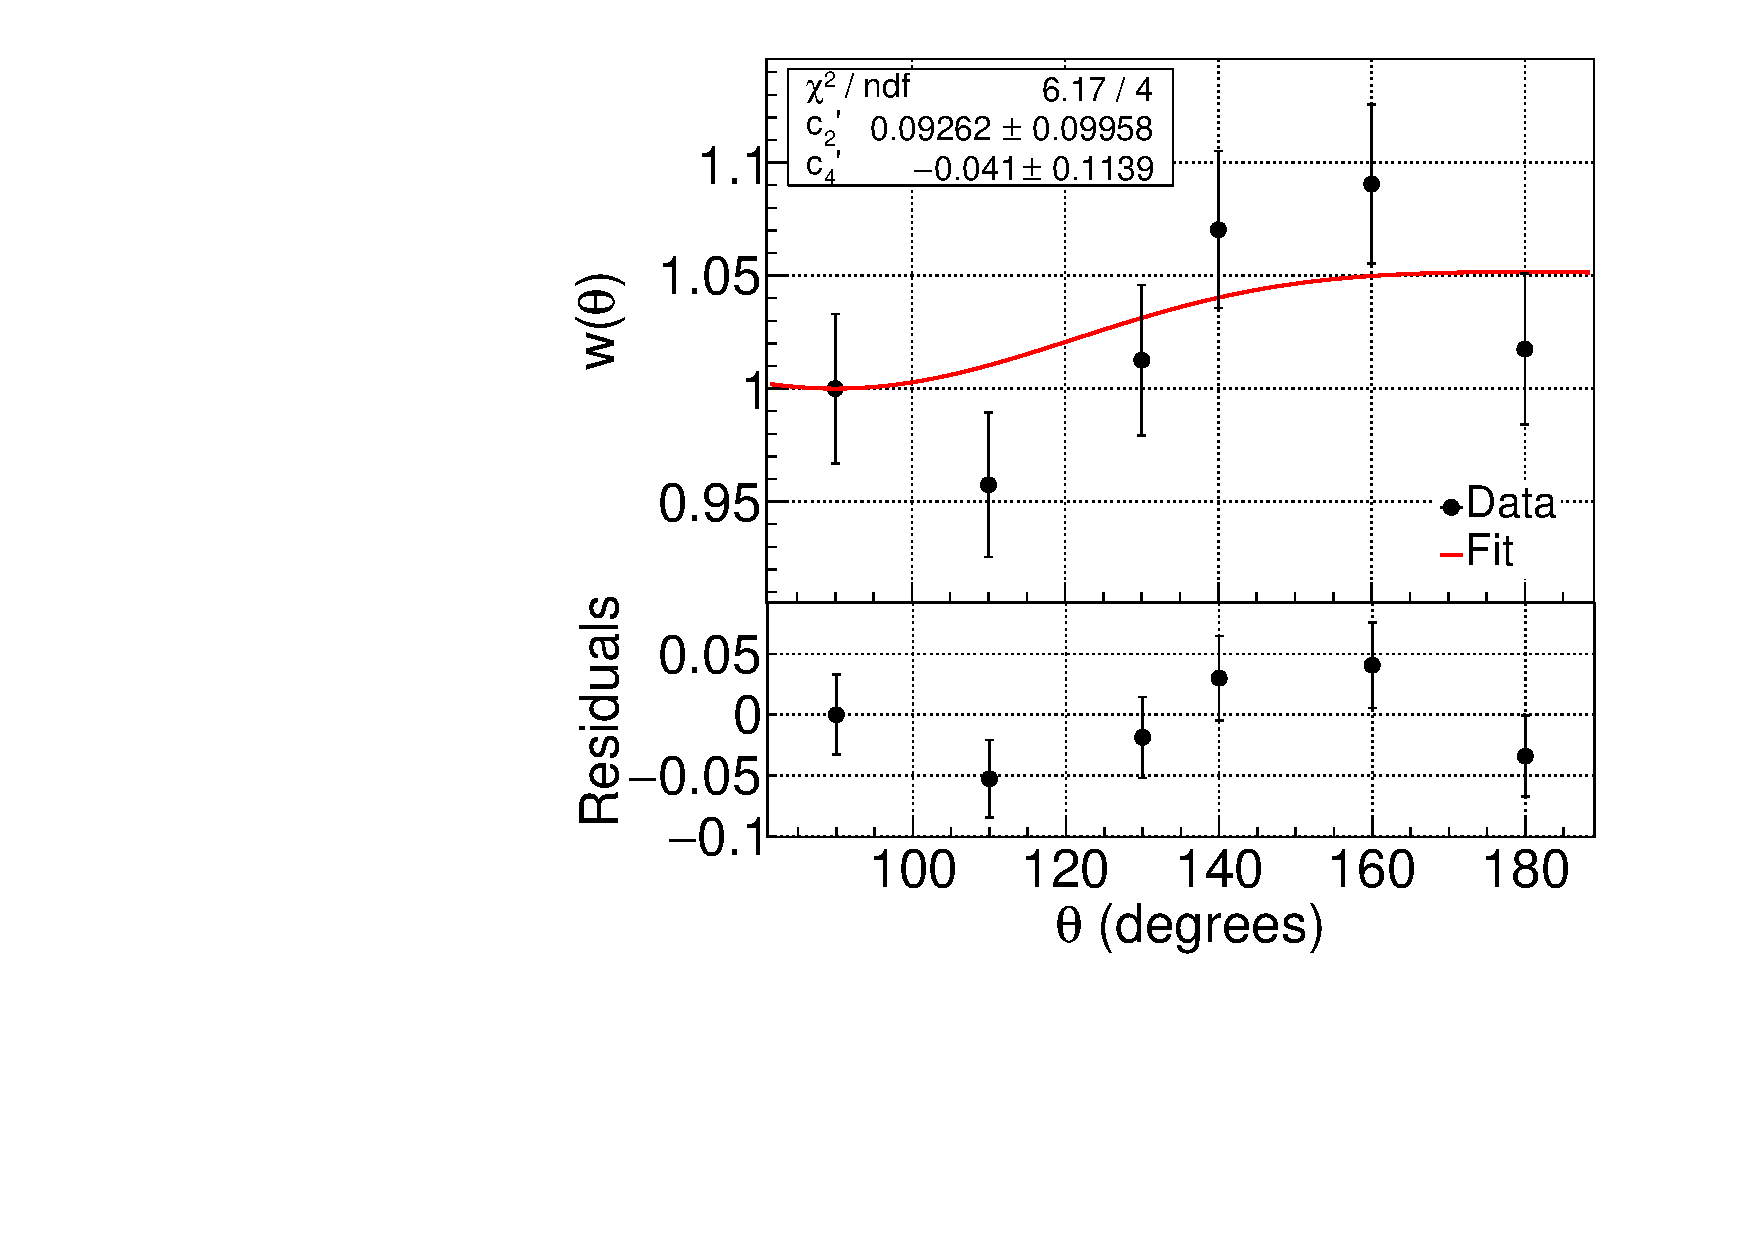
\includegraphics[width=0.58\linewidth]{Angular_Corr/residuals3.pdf}
    \hspace{-1cm}
    \caption{Angular correlation function: experimental data (see Tab. \ref{tab:angular corr function}) and fit according to Eq. \eqref{eq:w(theta)}}
    \label{fig: angular correlation function}
\end{figure}}
\end{table}
% \end{comment}

% \begin{figure}[H]
%     \centering
%     %\captionsetup{width=.5\linewidth}
%         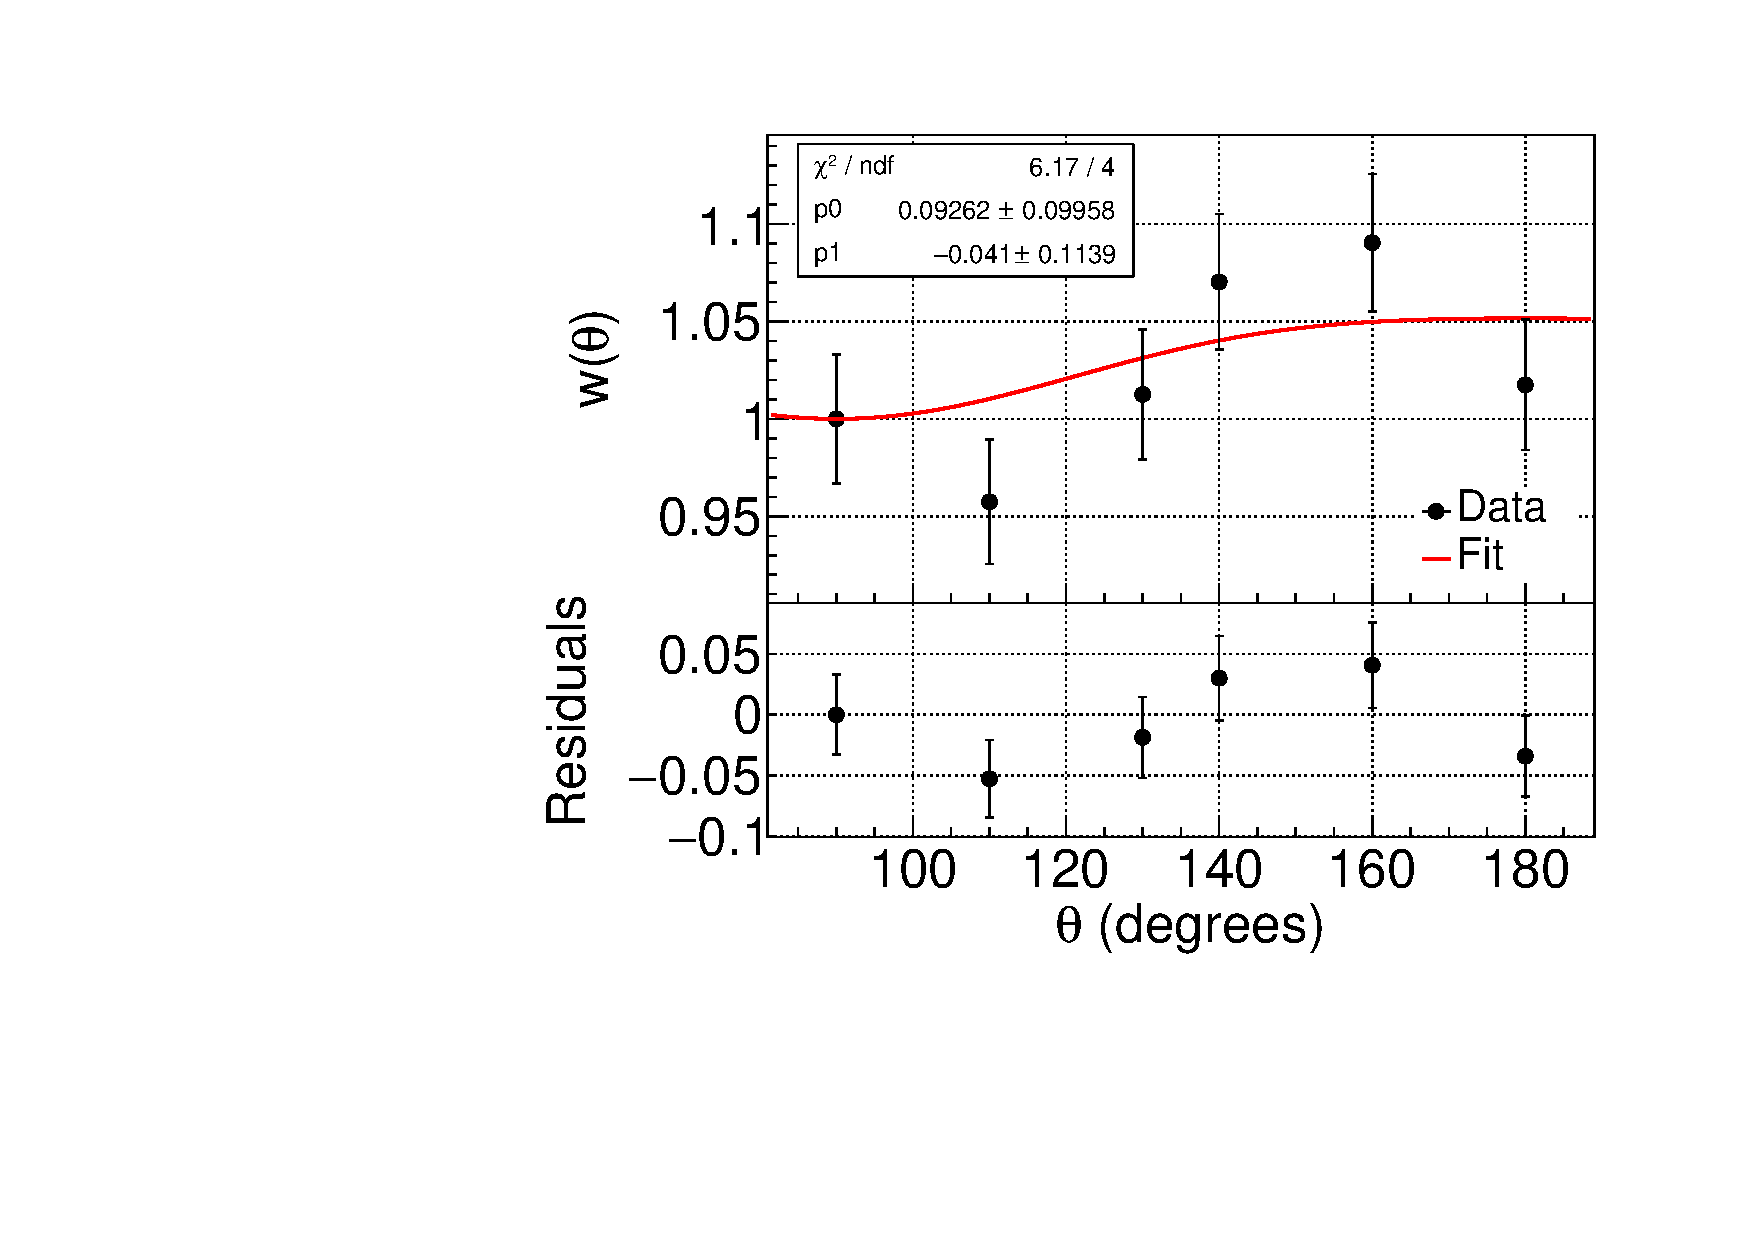
\includegraphics[width=0.48\linewidth]{Angular_Corr/residuals.pdf}
%         % \includegraphics[width=0.48\linewidth]{Angular_Corr/Ang_Corr_02_residual.pdf}
%     \caption{Fit of the angular correlation function with the experimental data.}
%     \label{fig: angular correlation function}
% \end{figure}

Let us perform a weighted least squares fitting procedure to the experimental data according to Eq. \eqref{eq:w(theta)}, using ROOT v. 6.30.08. The fitting curve (Fig. \ref{fig: angular correlation function}) turns out to have the following coefficients:
\begin{table}[H]
    \centering
    \begin{tabular}{|c|}
    \hline
    \[ c_2'=0.1\pm0.1\quad\quad \quad \quad c_4'=0.0\pm0.1\] \\
    \hline
    \end{tabular}
    %\caption{Caption}
    %\label{tab:my_label}
\end{table}
From the residual graph in Fig. \ref{fig: angular correlation function}, it might be seen that the agreement of the data trend with the fitting curve is not very good. In particular, the monotonicity of the curve is not respected over the sampled interval. As a consequence, the estimated coefficients have a high relative uncertainty. Nevertheless, due to large statistical uncertainties, the $\chi^2$ value does not allow us to reject the hypothesis with a confidence level higher than 81\%. 

The unexpected trend may be caused by several factors, such as an inaccurate selection of events, the presence of relevant angular correlations in the background or the low counting rate of events in D\#2. Besides, as explained in the previous Section, the possible systematic error introduced by an inaccurate source position cannot be effectively corrected. However, since that correction is expected to be relatively small, the effect cannot explain the observed trend.
%\textcolor{red}{read comment} %\textcolor{blue}{Do we want to hint at the strange repetition of total number of events among data sets as a factor decreasing our confidence in the counting of events?}\textcolor{red}{potremmo proporlo nelle conclusioni} M:ok

The estimated coefficients are lower than the theoretical ones. From a qualitative point of view, this is in agreement with the expectations because of geometrical corrections, but a quantitative comparison will not be performed here. %As for a quantitative comparison, instead, the geometrical corrections should be calculated as in \cite{0}. \textcolor{blue}{ [I have to change the numeration of the citations]}
    
\subsection{Detector efficiency measurements} \label{sect. efficiency}
This section is devoted to the assessment of the absolute peak efficiencies of the detectors. To do so, two independent methods will be employed using the same data acquisition. The acquisition consists of a $1\,\mathrm{h}\,\,47\,\mathrm{min}\,\,9\,\mathrm{s}$ 
%$\Delta t_\mathrm{source}=6429$ s 
run, divided into 11 runs (ten of 10 minutes each and one of 7.15 minutes), obtained with the "OR" trigger. 
The detectors were at 180° from each other, while their distances from the source were kept, as in the previous sections, at 31 cm for D\#2 and 12 cm for D\#1.
Moreover, another acquisition was recorded overnight in the same detectors and trigger configuration but in the absence of the source. 

Both methods are based on counting the events under the spectral peaks; the first exploits the $\gamma_a-\gamma_b$ coincidence in different detectors, whereas the second requires the coincidence to be in the same detector. 

Finally, the compatibility between these two methods will be analysed.

\subsubsection{Corrections for background and dead time losses}
First of all, let us subtract the background spectrum from the corresponding spectrum obtained in the presence of the source. The background spectra of the detectors must be normalized to the live time $\Delta t_\mathrm{source,live}$ of the acquisition recorded in the presence of the source, i.e. it must be rescaled by the factor
\[\frac{\Delta t_\mathrm{source,live}}{\Delta t_\mathrm{bkg}}\]
Here $\Delta t_\mathrm{bkg}=(71912.0\pm0.3)\,\mathrm{s}$ is the duration of the background acquisition and its uncertainty was estimated assuming a uniform probability within a maximum error of $1\,\mathrm{s}$. In the background acquisition the dead time of the counting system is negligible, because low counting rates are involved. 

As anticipated, in the presence of the source the real time $\Delta t_\mathrm{source}$ must instead be corrected for the dead time effect, so as to obtain the live time:
\[\Delta t_\mathrm{source,live}=\Delta t_\mathrm{source}-\Delta t_\mathrm{source,dead}\]
The real time is $\Delta t_\mathrm{source}=(6429.0\pm0.1)\,\mathrm{s}$, where the uncertainty now assumes a maximum error of $0.5\;\mathrm{s}$. 
In order to estimate $\Delta t_\mathrm{source,dead}$, the number of events seen by the digitizer was compared with the number of events read by the CAEN scaler during the same "OR" run, which lasted 3 min. 
Contrary to the expectations, the digitizer counting, 1766752 events, turns out to be higher than the scaler one, 1720759 events. The cause might be a problem in the scaler settings or in the digitizer treatment of saturated signals. 
Since the dead time cannot be determined from those measurements, let us use the dead time estimation performed by CoMPASS\footnote{Since the estimation for some runs was not stable, we assume that the uncertainty here is the one of a uniform distribution within a maximum error of 0.1\%.}: $(0.50\pm0.03)\%$ in the acquisition recorded in the presence of the source. Hence, the corresponding live time is 
$\Delta t_\mathrm{source,live}=(1-0.5\%)\Delta t_\mathrm{source}=(6397\pm2)\,\mathrm{s}$.

%In order to have a precise analysis of the detector efficiency is important to consider the effect of the dead time of the Digitizer. Indeed, the digitizer requires more time to acquire data and it's possible to evaluate this time by comparing the number of events seen by the digitizer with the number of events read by the CAEN scaler of the same run. To do that, a 3 min of acquisition was taken with detectors in … (position). Again, a source of \ce{^60}Co was used.


Now let us plot in Fig. \ref{fig:spectra with background 1st calibration} the original "total" spectrum recorded in the presence of the source (blue), the normalized background spectrum (green) and the difference of the two (red). The left panel refers to D\#1, while the right one to D\#2. For each detector, both the blue and the green spectra are calibrated according to the corresponding expression found in Sect. \ref{sect:energy calibration}. 

\begin{figure}[H]
    \centering
    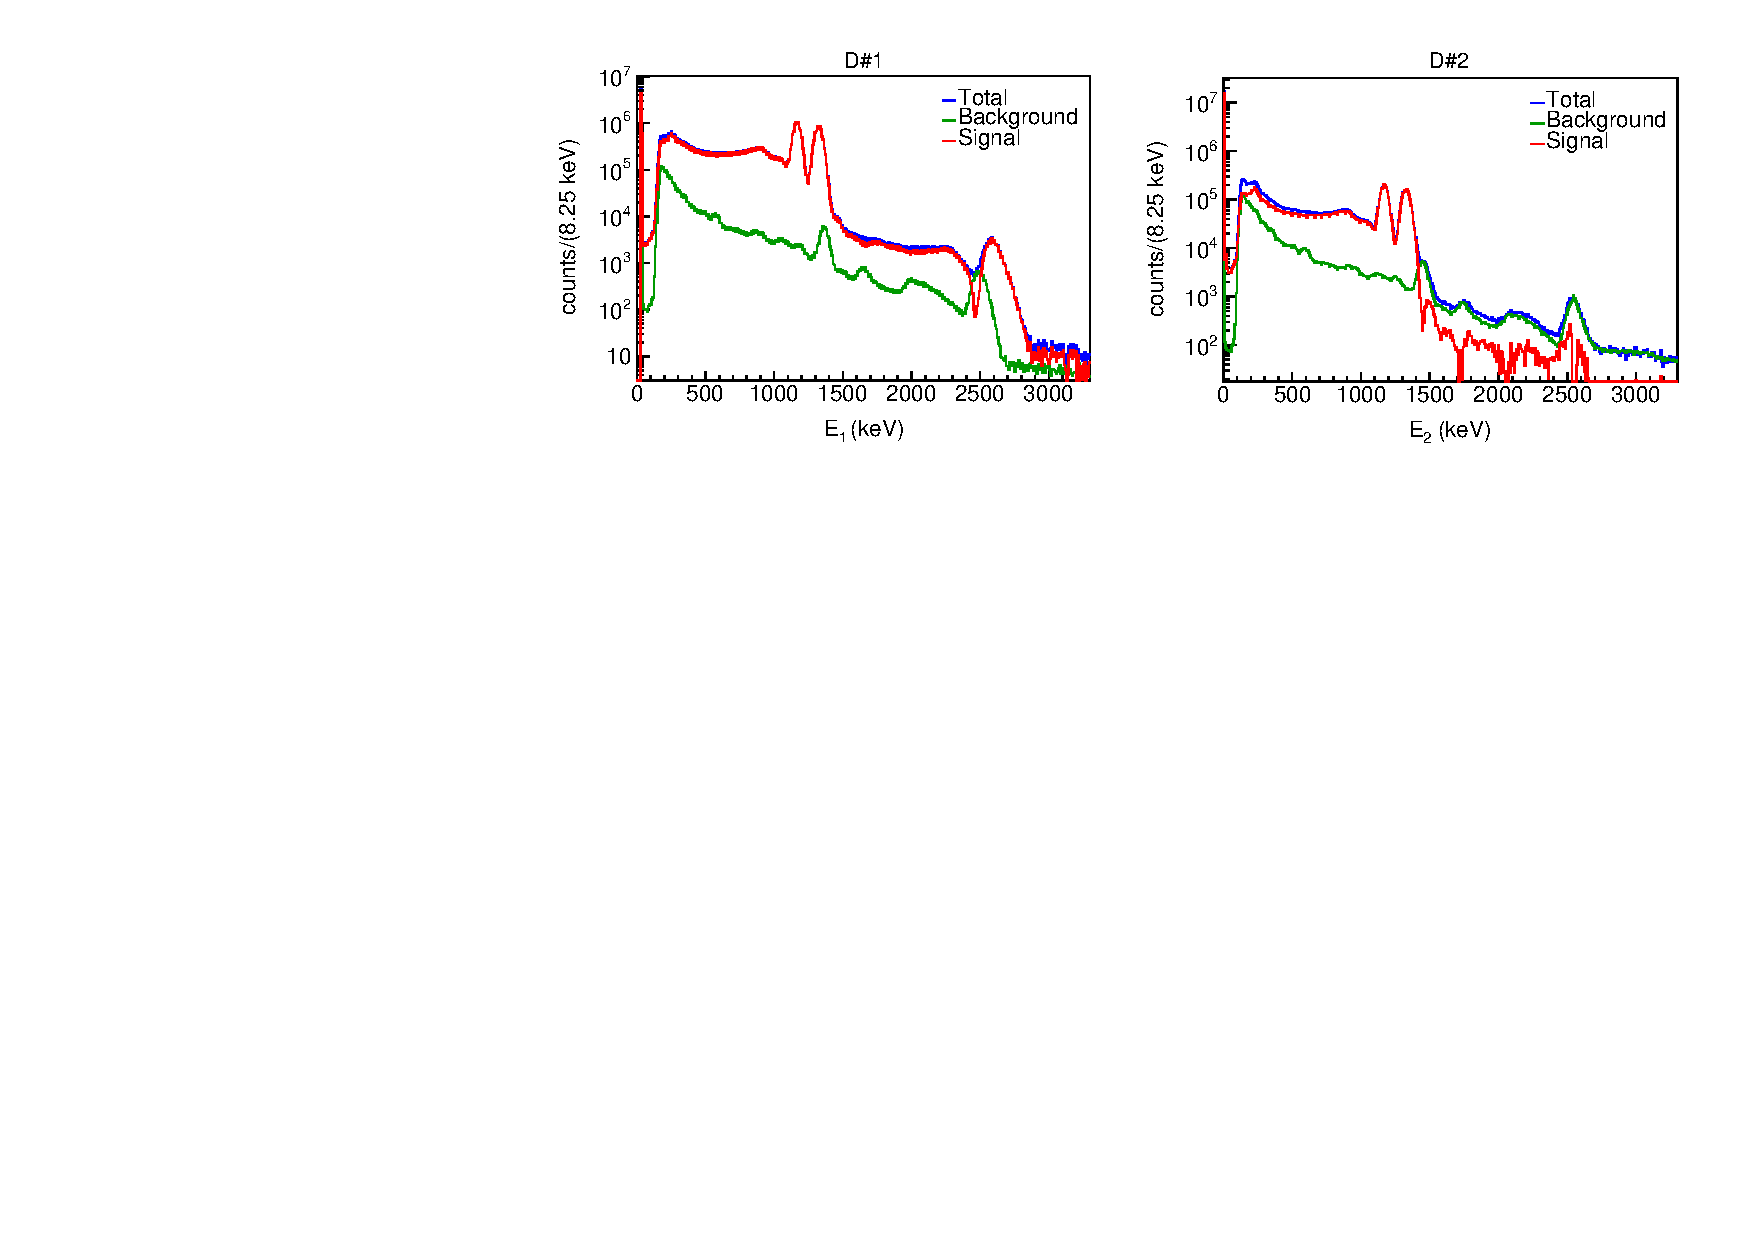
\includegraphics[width=1.0\linewidth]{Efficiency/Prova9.pdf}
    \caption{Spectrum recorded in the presence of the source (blue), background normalized spectrum (green) and difference of the two (red) for D\#1 (left) and D\#2 (right). In each panel, all the spectra are calibrated with the calibrations found in Sect. \ref{sect:energy calibration}.}
    \label{fig:spectra with background 1st calibration}
\end{figure}

It is apparent that in D\#2 the entries with an energy higher than $E_b$ are mainly due to background radiation, so the counting rate in detector \#2 is too low to observe the sum peak clearly. 
Moreover, when looking at the peaks in the background spectra, one might see that their calibration in D\#1 is not the same as in D\#2. In particular, the \ce{^40}K peak is placed at $\approx\!1350$ keV in D\#1 and $\approx\!1450$ keV in D\#2, whereas its nominal value is $1460$ keV. Furthermore, in the spectrum on the left of Fig. \ref{fig:spectra with background 1st calibration}, for D\#1, the sum peak is not centred at the expected value, but at a significantly higher one, and this effect does not seem due to the sum of other events. Not only does the energy calibration of D\#1 seem to fail at high energies, but also it seems that in D\#1 the background spectrum and the total spectrum do not share the same calibration. 

Let us calibrate again the spectra of D\#1, performing now two different channel-energy calibrations, one for the total spectrum and one for the background spectrum. In particular,

\begin{itemize}
    \item[-] as for the total spectrum, let us consider the 1173 and 1332 keV peaks, together with the 2506 sum peak. Besides, let us perform an unweighted linear fit, because a weighted fit would almost neglect the last point, being its position uncertainty much higher then the previous two;
    \item[-] as for the background spectrum, let us consider the \ce{^40}K peak and the  \ce{^208}Tl peak, which correspond to 1460 keV and 2573 keV respectively.
\end{itemize}
The new conversion relations for D\#1 are 

\begin{comment}
\begin{align}
    \text{Total:}&\quad\mathrm{channel}=(0.982\pm0.008)\mathrm{\tfrac{ch}{keV}}\cdot E_1+(-110\pm10)\,\mathrm{ch}\\
    \text{Background:}&\quad\mathrm{channel}=(0.9332\pm0.0002)\mathrm{\tfrac{ch}{keV}}\cdot E_1+(-137.1\pm0.3)\,\mathrm{ch}
\end{align}
\end{comment}

\begin{table}[H]
    \centering
    \begin{tabular}{|l|cc|}
    \hline
     Total & $m_1'=(0.982\pm0.008)\,\frac{\mathrm{ch}}{\mathrm{keV}}$ &  $q_1'=(-110\pm10) \,\mathrm{ch}$\\
     Background & $m_{1,\mathrm{bkg}}=(0.9332\pm0.0002)\,\frac{\mathrm{ch}}{\mathrm{keV}}$ & $q_{1,\mathrm{bkg}}=(-137.1\pm0.3)\,\mathrm{ch}$\\ 
    \hline        
    \end{tabular}
    \caption{Fit parameters for new energy calibration of D\#1}%: total is obtained using also the sum peak, background referres to the new parameters for D\#1 background}
    \label{tab:cal_fit_new}
\end{table}


Figure \ref{fig:spectra with background 2nd calibration} shows the total, background and signal histograms of D\#1 with the new calibrations.
\begin{figure}[H]
    \centering
    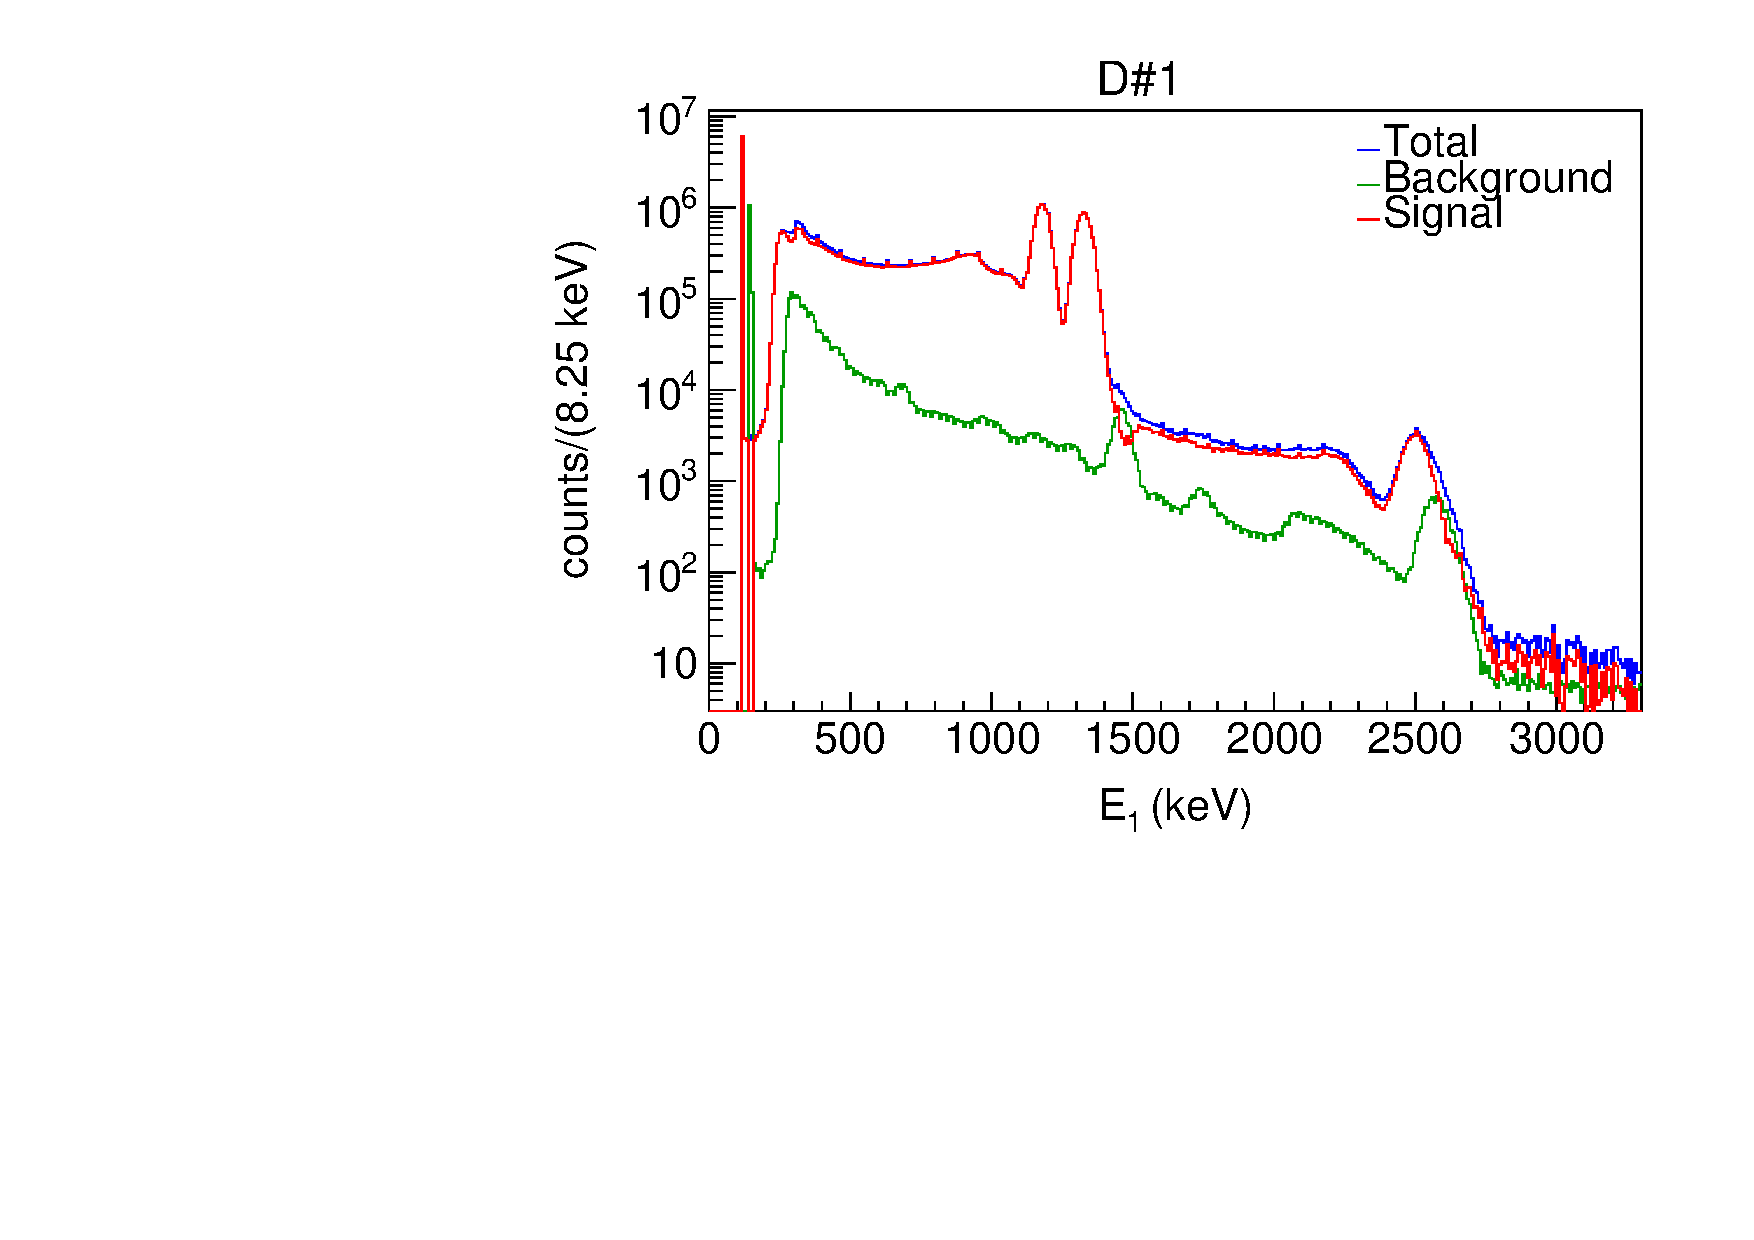
\includegraphics[width=0.5\linewidth]{Efficiency/2calibrations_d1_2.pdf}
    \caption{Same spectra as in Fig. \ref{fig:spectra with background 1st calibration} for D\#1, but calibrated as explained above}
    \label{fig:spectra with background 2nd calibration}
\end{figure}

\subsubsection{Coincidence method}
As introduced at the beginning of Sect. \ref{sect. efficiency}, the first method is based on the counting of coincidence events under the two peaks of $1173\,\mathrm{eV}$ and $1332\,\mathrm{keV}$ in different detectors. In particular, the method exploits the number of events in which one $\gamma$-ray is detected in one detector and the other coincidence $\gamma$-ray is detected in the other detector. %This method is based on the assumption that if a photon with one of these energies has been seen in one of the detector, another photon of the other energy must be seen on the other detector. \\
Since the method requires a two-dimensional analysis of coincidence events, let us plot in Fig. \ref{fig:coincidence method} the correlation between the energies released in the detectors, calibrated as explained in the previous paragraph.
\begin{figure}[H]
    \centering
    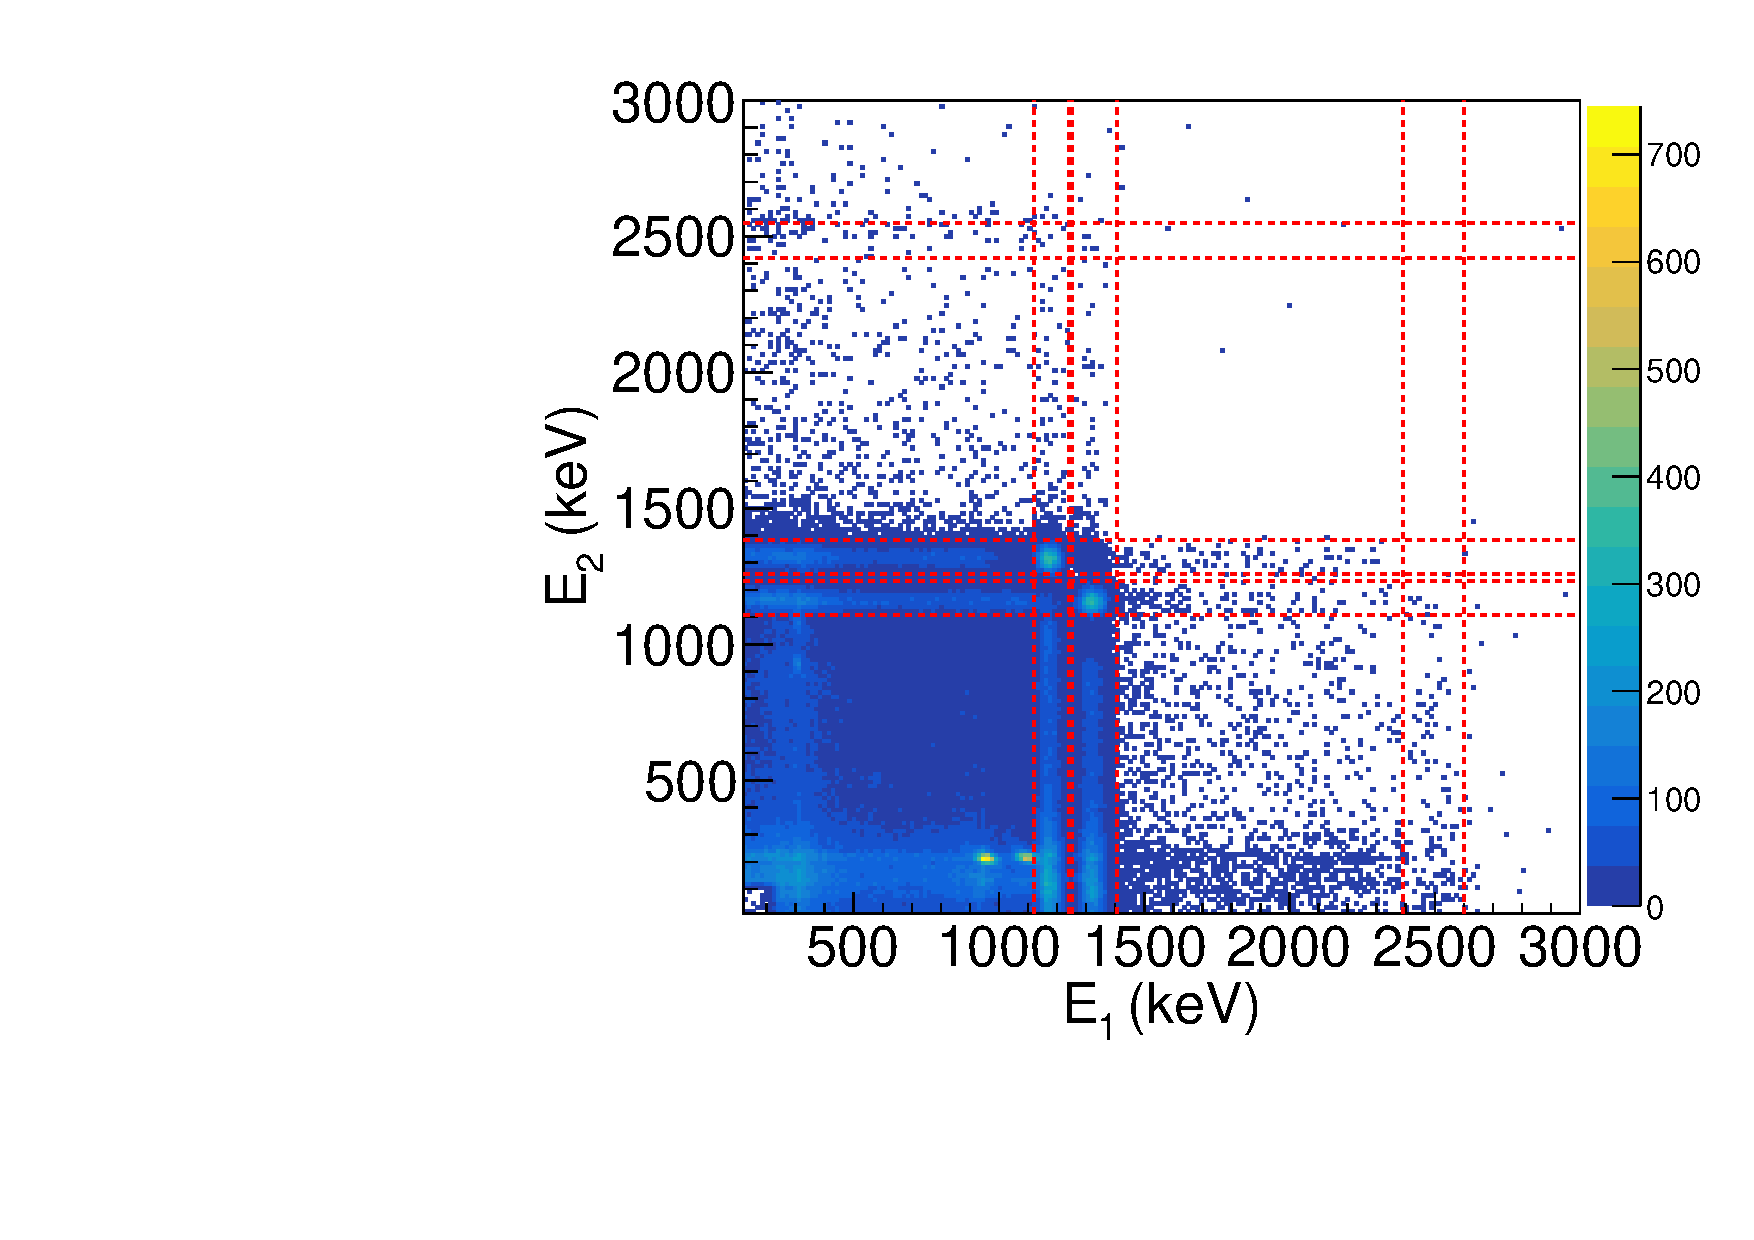
\includegraphics[width=0.5\linewidth]{Efficiency/h3_g.pdf}
    \caption{Correlation between the "total" energy spectra of D\#1 and D\#2, excluding the events with energy close to zero. The energy $E_1$ is calibrated with the new calibration. The dashed red lines highlight the integration intervals (Tab. \ref{tab:integration limits}) used for both methods. In particular, the three small squares around 1300 keV were used to select the coincidence events for the coincidence method.}
    \label{fig:coincidence method}
\end{figure}

Firstly, in order to count the events, let us select proper intervals to distinguish the first and the second peak in each detector (Tab. \ref{tab:integration limits}, first two columns). Those will be kept fixed for the entire study of the efficiency (then, also for the sum peak method in Sect. \ref{sect: sum peak}). The selected intervals can be seen in Fig. \ref{fig:coincidence method}, following the red lines.
\begin{table}[H]
    \centering
    \begin{tabular}{|l|ccc|}
    \hline
       & $E_a$ (keV) & $E_b$ (keV) & $E_a+E_b$ (keV)\\
       \hline
       D\#1 & [1120;1242] & [1253;1405] & [2390;2600]\\
       D\#2 & [1106;1232] & [1257;1383] & [2420;2550]\\
       \hline
    \end{tabular}
    \caption{Integration extremes used for selection of $E_a$, $E_b$ and $E_a+E_b$ peaks in D\#1 and in D\#2}
    \label{tab:integration limits}
\end{table}

It is now possible to count the events under the relevant peaks: the events under a peak were selected and counted ($N_i(E_j)$, with $i=1,2$ detector number and $j=a,b$ peak name) for a detector and then the events under the other peak in the other detector were counted ($N(E_k;E_j)$, $j,k=a,b$, where the first and second terms in parentheses correspond to D\#1 and D\#2 respectively). %\footnote{The number on the subindex indicates the detectors and the energies in the brackets the energy of the peak. Notation $N_{1}(E_a;E_b)$ indicates the number of events registered by D\#1 with energy $E_a$, after fixing the events with energy $E_b$ on D\#2, and so on. Those are expected to be the same, so redefined as $N(E_k;E_j)$.}).
The results are given in the following table (Tab. \ref{tab: coincidence method}); the uncertainties on the number of events consider both the error associated to the statistic of Poisson and the uncertainties on the acquisition time.

Let's remind also that the spectra used in these sections are all calibrated and the background, as explained before, has been subtracted from each spectrum (as in Fig. \ref{fig:spectra with background 1st calibration} and \ref{fig:spectra with background 2nd calibration}).  Moreover, from the first peak, with energy centred at $E_a=1173\,\mathrm{keV}$, the continuum has been subtracted by performing a linear interpolation between the values on either side of the peak. %\textcolor{red}{vedi tu se vuoi aggiungere qualcosa}

\begin{comment}
\begin{table}[H]
    \centering
    \begin{tabular}{|l|cc|cc|cc|}
    \hline
        & \multicolumn{2}{c|}{$E_a$} & \multicolumn{2}{c|}{$E_b$} & \multicolumn{2}{c|}{$E_a+E_b$}\\
       \cline{2 - 7}
       &left&right& left&right &left&right\\
       &(keV)&(keV)&(keV)& (keV)& (keV)& (keV) \\
       \hline
       D\#1 1120 & 1242
       D\#2 \
       \hline
    \end{tabular}
    \caption{Integration extremes used for selection of $E_a$, $E_b$ and $E_a+E_b$ peaks in D\#1 and in D\#2}
    \label{tab:integration limits}
\end{table}
\end{comment}



% \begin{table}[H]
%     \centering
%     \begin{tabular}{|c|c|c|}
%     \hline
%       & D\#1 &  D\#2\\
%     \hline
%        $N_1(E_a)= (8.617\pm0.003)\cdot10^6 $& $N_{1}(E_a;E_b)= (7.48\pm0.09)\cdot10^3$ & $N_{2}(E_a;E_b)=(8.20\pm0.09)\cdot10^3$\\ 
%        $N_1(E_b)= (7.464\pm0.003)\cdot10^6$& $N_{1}(E_b;E_a)=(8.40\pm0.09)\cdot10^3$ & $N_{2}(E_b;E_a)=(2.77\pm0.05)\cdot10^3$\\
%        $N_2(E_a)= (1.746\pm0.001)\cdot10^6$& $N_{1}(E_b;E_b)=450\pm20$ & $N_{2}(E_b;E_b)= 500\pm20 $\\
%        $N_2(E_b)= (1.315\pm0.001)\cdot10^6$& & \\
%          \hline
%     \end{tabular}
%     \caption{Coincidence method counts}
%     \label{tab: coincidence method}
% \end{table}
\begin{comment}
    \begin{table}[H]
    \centering
    \begin{tabular}{|l|cc|}
    \hline
        &Counts D\#1&Counts D\#2\\
        \hline
        $N_i(E_a)$ & $(8.661\pm0.003)\cdot10^6$ &$(1.755\pm0.001)\cdot10^6$\\
        $N_i(E_b)$ &$(7.502\pm0.003)\cdot10^6$ &$(1.456\pm0.001)\cdot10^6$\\
        \hline
         &\multicolumn{2}{c|}{Coincidence counts}\\
         \hline
       $N(E_a;E_b)$ &\multicolumn{2}{c|}{$(8.24\pm0.09)\cdot10^3$}\\
       $N(E_b;E_a)$ &\multicolumn{2}{c|}{$(8.44\pm0.09)\cdot10^3$}\\
       $N(E_b;E_b)$ &\multicolumn{2}{c|}{$(0.50\pm0.02)\cdot10^3$} \\
       \hline
    \end{tabular}
    \caption{\textcolor{blue}{Ho messo in appendice le equazioni di partenza, ammesso che siano giuste. Se vuoi puoi fare riferimento a quelle per descrivere le varie grandezze. I've written the counts in the excel file, but it would be better to check them}}
    \label{tab: coincidence method}
\end{table}
\end{comment}

\begin{table}[H]
    \centering
    \begin{tabular}{|l|cc|}
    \hline
        &Counts D\#1&Counts D\#2\\
        \hline
        $N_i(E_a)$ & $(8.456\pm0.003)\cdot10^6$ &$(1.683\pm0.001)\cdot10^6$\\
        $N_i(E_b)$ &$(7.468\pm0.003)\cdot10^6$ &$(1.430\pm0.001)\cdot10^6$\\
        \hline
         &\multicolumn{2}{c|}{Coincidence counts}\\
         \hline
       $N(E_a;E_b)$ &\multicolumn{2}{c|}{$(8.24\pm0.09)\cdot10^3$}\\
       $N(E_b;E_a)$ &\multicolumn{2}{c|}{$(8.44\pm0.09)\cdot10^3$}\\
       $N(E_b;E_b)$ &\multicolumn{2}{c|}{$(0.50\pm0.02)\cdot10^3$} \\
       \hline
    \end{tabular}
    \caption{Coincidence method counts}
    \label{tab: coincidence method}
    %\textcolor{blue}{Ho messo in appendice le equazioni di partenza, ammesso che siano giuste. Se vuoi puoi fare riferimento a quelle per descrivere le varie grandezze.}
    \label{tab: coincidence method}
\end{table}


%sistematic errors: Sometimes the same detector could see two photons 
Therefore, with this method, four different terms related to efficiency can be evaluated:
\begin{itemize}
    \item [-] $\varepsilon_{1}(E_a)=$ peak efficiency of the detector 1 on detecting $\gamma_a$, i.e. photon with $E_a=1173\,\mathrm{keV}$;
    \item[-] $\varepsilon_{1}(E_b)=$ peak efficiency of the detector 1 on detecting $\gamma_b$, i.e. photon with $E_b=1332\,\mathrm{keV}$;
    \item [-] $\varepsilon_{2}(E_a)=$ peak efficiency of the detector 2 on detecting $\gamma_a$, i.e. photon with $E_a=1173\,\mathrm{keV}$;
    \item[-] $\varepsilon_{2}
    (E_b)=$ peak efficiency of the detector 2 on detecting $\gamma_b$, i.e. photon with $E_b=1332\,\mathrm{keV}$.
\end{itemize}

These terms are calculated as follows. In the denominator, %first term
the events attributable to the systematic error of chance coincidence, $N_\mathrm{ch}$ or $N_\mathrm{ch}'$. %($N(E_b;E_b)$) 
are subtracted from the corresponding counted coincidence events. Then, the result is divided also by a factor $w(180^\circ)$, estimated in Sect. \ref{sect: angular}. These formulae may be derived from the ones written in Appendix.
\vspace{-0.3cm}
\begin{multicols}{2}
\begin{subequations}
    %\begin{align}
     \begin{empheq}[left={\empheqlbrace\,}]{align}
& \varepsilon_{1}(E_a)=\frac{N(E_a;\,
E_b)-N_\mathrm{ch}}{N_2(E_b)\,w(180^\circ)} \label{eq: sub, coinc1}\\
&\varepsilon_{1}(E_b)=\frac{N(E_b;\, E_a)-N'_\mathrm{ch}}{N_2(E_a)\,w(180^\circ)} \label{eq: sub, coinc1}
%\end{align}
\end{empheq}
\end{subequations}

\begin{subequations}
    %\begin{align}
     \begin{empheq}[left={\empheqlbrace\,}]{align}
& \varepsilon_{2}(E_a)=\frac{N(E_b;\,
E_a)-N'_\mathrm{ch}}{N_1(E_b)\,w(180^\circ)} \\
&\varepsilon_{2}(E_b)=\frac{N(E_a;\, E_b)-N_\mathrm{ch}}{N_1(E_a)\,w(180^\circ)} 
%\end{align}
\end{empheq}
\end{subequations}
\end{multicols}

The chance coincidence correction can be estimated exploiting the fact that the chance coincidence rate is proportional to the product of the rates of the events creating the coincidence; using the measurement of the $N(E_b;E_b)$ events (presented in Tab. \ref{tab: coincidence method}), the following estimates can be made:
% \begin{equation}
%     N_\mathrm{ch}\approx N(E_b;\,E_b)
% \end{equation}
\begin{equation}
    N_{\mathrm{ch}}=\frac{N_1(E_a)N(E_b;E_b)}{N_1(E_b)}\approx N(E_b;E_b)\,,\quad\quad\quad    N_{\mathrm{ch}}'=\frac{N_2(E_a)N(E_b;E_b)}{N_2(E_b)}\approx N(E_b;E_b)
\end{equation}
%explanation of the formulas (mi sembrano abbastanza chiare, basta spiegare il termine N_ch and w) and calculation.

The results are shown in the next table.
\begin{table}[H]
    \centering
    \begin{tabular}{|c|cc|}
         \hline
         & D\#1&D\#2\\
         \hline
          $\varepsilon(E_a)$&$(0.53\pm0.02)\%$ & $(0.102\pm0.003)\%$ \\
          %$(0.56\pm0.02)\%$ & $(0.111\pm0.003)\%$  \\
          $\varepsilon(E_b)$&$(0.46\pm0.01)\%$ & $(0.092\pm0.003)\%$ \\
          %$(0.48\pm0.02)\%$ & $(0.094\pm0.003)\%$ \\
          \hline
    \end{tabular}
    \caption{Detector absolute peak efficiencies estimated with the coincidence method}
    \label{tab:coinc_results}
\end{table}
Let us notice that the uncertainties of these measurements are underestimated, because they have been calculated taking into account only counting statistics as a source of uncertainty in counting the events. Other possible sources, however, may be relevant and cause a systematic error; they are for example the arbitrariness of the choice of the integration extremes, the role of the energy calibration of the background or the method used to estimate the continuum.

\subsubsection{Sum peak method}\label{sect: sum peak}
The sum peak method is based on the probability of detecting both $\gamma$s in the same detector: % i.e. to have a retro-diffused photon.  
since the two photons from the same nucleus are emitted so close in time to be considered in coincidence, this event will provide a peak (\textit{sum peak}) centred at an energy value which is the sum of the two energies of the photons, $2505\,\mathrm{keV}$.

%SISTEMATIC ERROR PEAKS
The method relies on the determination of the areas of the 1173, 1332 and 2505 peaks in the \ce{^60}Co spectrum, together with the area of the integral spectrum. In fact, the peak areas depend on the efficiencies at those energies. 
If one approximates the emission probability of the two $\gamma$s as 100\%, in a first approximation the equations presented in the Appendix can be written. Neglecting for the moment the chance coincidence term $N_{\mathrm{\Sigma,ch},i}$ and solving the equations, it is possible to show that the absolute peak efficiencies of detector number $i=1,2$ can be calculated as:
\begin{equation}\label{eq: efficiency sum peak}
    \varepsilon_{i}(E_a)=\frac{N_i(E_a\!+\!E_b)}{w(0^\circ)\big(N_i(E_b)+\frac{N_i(E_a\!+\!E_b)}{r_i}\big)}\,,\quad\quad\quad
    \varepsilon_{i}(E_b)=\frac{N_i(E_a\!+\!E_b)}{w(0^\circ)\big(N_i(E_a)+\frac{N_i(E_a\!+\!E_b)}{r_i}\big)}
\end{equation}
Again, $N_i(E)$ is the number of counts under the peak at energy $E$ in detector $\#i$. The quantity $r_i$ is the peak-to-total ratio of detector $\#i$; in principle it should depend on the energy $E$ of the peak taken into account, but let us estimate it as
\begin{equation} \label{eq:peak to total ratio}
    r_i\approx\frac{N_i(E_a)+N_i(E_b)}{N_{\mathrm{tot},i}}
\end{equation}
where $N_{\mathrm{tot},i}$ is the total number of events in the spectrum of detector $\#i$.
The factor $w(0^\circ)$, instead, corrects for the $\gamma-\gamma$ angular correlation, i.e. for the relative probability of both $\gamma$s to be emitted in the same direction. Since the theoretical angular correlation function introduced in Sect. \ref{sect: angular} is periodic with period $\pi$, it is expected $w(0^\circ)\!=\!w(180^\circ)$, so let us use again the experimental point $w(180^\circ)$ presented in Sect. \ref{sect: angular} as an estimation of $w(0^\circ)$.

The quantities $N_i(E_a)$ and $N_i(E_b)$, for both $i=1,2$, have already been calculated in the previous section and are listed in Tab. \ref{tab: coincidence method}. The number of events under the sum peak of detector $\#i$, $N_i(E_a\!+\!E_b)$, can be determined similarly, selecting the events in the intervals shown in Tab. \ref{tab:integration limits}. 
As for the total number of events in detector $\#i$ after background subtraction, $N_{\mathrm{tot},i}$, let us remember that the trigger of the acquisition was the "OR" of the detectors. Thus, for each detector let us exclude the events whose energy is close to zero, because they occurred only in the other detector. In particular, the excluded events are those with energy less than 150 keV in D\#1 and less than 30 keV in D\#2. 
The results of these new counts are presented in Tab. \ref{tab:sum peak method}. Using Eq. \eqref{eq: efficiency sum peak}-\eqref{eq:peak to total ratio}, let us now estimate the peak efficiencies, shown in Tab. \ref{tab:sum_results}.
\begin{table}[H]
    \centering
    \begin{tabular}{|c|cc|}
    \hline
       %  & \multicolumn{2}{c|}{D\#1}&\multicolumn{2}{c|}{D\#2}\\
       &Counts D\#1 &Counts D\#2\\
       \hline
       $N_i(E_a\!+\!E_b)$ & $(4.46\pm0.2)\cdot10^4$ &$(1.47\pm0.09)\cdot10^3$ \\
        $N_{\mathrm{tot},i}$& $(5.3515\pm0.0008)\cdot 10^7$&$(2.6681\pm0.0006)\cdot 10^7$\\
       \hline
    \end{tabular}
    \caption{Counts for the sum peak method: sum peak counts and total counts in the spectrum of detector $\#i=1,2$. For $N_i(E_a)$ and $N_i(E_b)$ see Tab. \ref{tab: coincidence method}.}
    \label{tab:sum peak method}
\end{table}

\begin{table}[H]
    \centering
    \begin{tabular}{|c|cc|}
         \hline
         & D\#1&D\#2\\
         \hline
          $\varepsilon(E_a)$&$(0.57\pm0.02)\%$ & $(0.100\pm0.007)\%$ \\
          $\varepsilon(E_b)$&$(0.50\pm0.01)\%$ & $(0.083\pm0.006)\%$ \\
          \hline
    \end{tabular}
    \caption{Detector absolute peak efficiencies estimated with the sum peak method}
    \label{tab:sum_results}
\end{table}
The same considerations about the uncertainties hold as in the coincidence method case. In this method, a further factor that tends to increase the error is the difficulty in the estimation of the total count rate, which requires an accurate knowledge of the background, the exclusion of the "OR" events that occurred in the other detector and in principle also a reconstruction of the counts below the LLD.
\paragraph{Correction for random summing effect}
In order to correct for the random summing effect, i.e. events in the sum peak created by two $\gamma$s produced in two different decays, the chance coincidence contribution should be removed from the sum peak counts. For a given detector, this contribution to the sum peak can be expressed as
\begin{equation}
    N_\mathrm{\Sigma,ch}=2\sqrt{N(2\,E_a)\,N(2\,E_b)}
\end{equation}
where $N(2E_a)$ and $N(2E_b)$ are the areas of the peaks at $2\times 1173$ and $2\times1332$ keV. In fact, the chance coincidence rate is proportional to the product of the rates of the events creating the coincidence and the random sum peak has two possible combinations of events, i.e. $1173+1332$ or $1332+1173$. 
However, in our spectra, even if the background has been subtracted, no such peaks are visible. %, as one might see in Fig. \ref{fig:around 2506 keV}. 
Hence, this correction will be neglected.
% \begin{figure}[H]
%     \centering
%     \includegraphics[width=1.0\linewidth]{}
%     \caption{Zoom around the sum peak in D\#1 (left) and D\#2 (right): the peaks at $2\times 1173$ and $2\times 1332$ keV are not visible in either detector.}
%     \label{fig:around 2506 keV}
% \end{figure}

\subsubsection{Compatibility of the two methods and final result}
%COMPATIBILITà TRA I METODI
%STIMA FINALE
%COMMENTO
Let us now perform a brief compatibility analysis of the efficiencies obtained with the two methods. The compatibility coefficients between the previous estimates (Tab. \ref{tab:compatibilities and means}) show that the results from the two methods are consistent with each other, despite the fact that the uncertainties are probably underestimated. However, we do not perform a weighted average between the two methods because this would further reduce the uncertainties.
\begin{table}[H]
    \centering
    \captionsetup{width=0.85\linewidth}
    \begin{tabular}{|l|cc|cc|}
         \hline
         & $\varepsilon_{1}(E_a)$&$\varepsilon_{1}(E_b)$&$\varepsilon_{2}(E_a)$& $\varepsilon_{2}(E_b)$\\
         \hline
          Compatibility& 1.4&2.8&0.3&1.0\\
          \hline
    \end{tabular}
    \caption{Compatibility indexes between the results $\varepsilon_{i}(E_j)$ of the peak efficiencies estimated with the two methods: coincidence and sum peak.}
    \label{tab:compatibilities and means}
\end{table}


\section{Results and conclusions}
The analysis of the position of the source %(Sect. \ref{position})
has revealed that the source was not centred on the support, but those results could not be used to correct the angular correlation measurements because the source position had changed between the two measurement parts. 

The points of the angular correlation function (Fig. \ref{fig: angular correlation function}) have been determined by selecting particular coincidence events of "AND" acquisitions at different angles. The points do not follow exactly the expected function. %The uncertainties on the fit parameters are big enough to be considered compatible, but the difference from the expected results is clear.%penso che neanche in teoria debbano essere compatibili per le correzioni dovute all'angolo solido. Non so però quanto dovrebbero venire nelle condizioni geometriche nostre
The possible causes have been listed in the related paragraph.

As for the detection efficiencies, they have been calculated starting from the counting measurements in the spectra recorded in a long "OR" acquisition, after normalized background subtraction (Fig. \ref{fig:spectra with background 2nd calibration} for D\#1 and Fig. \ref{fig:spectra with background 1st calibration} on the right for D\#2). In particular, the net peak areas, the two-dimensional coincidence counts and the sum peak coincidence counts have been calculated. The two methods have shown compatible results (Tables \ref{tab:coinc_results} and \ref{tab:sum peak method}), despite a possible underestimation of their uncertainties. %, which also seems to be lower than expected. %Secondo me se non presentiamo una stima a priori non possiamo dire che sono troppo basse
In both methods the angular correlation correction has been introduced using the previous measurements. While for the first method it has been possible to estimate the chance coincidence correction, for the second one it has not been possible to correct for the effect of chance summing systematic error because the spectra have not shown the expected peaks at energies $2\times1173$ keV and $2\times1332$ keV.\\

\noindent
To conclude, let us suggest some observations about the measuring procedure and the stability of the digitizer energy and counting measurements. %Indeed, those turn out to be unstable in some situation.

The distance of the second detector from the source was chosen that big in order to reduce the impact of a possible miscentering of the source. However, later that distance has turned up to be too big, because it has caused a very poor statistics of signal events in the energy region of the sum peak of D\#2. Thus, a significant improvement may be achieved by bringing the second detector closer.

The energy calibration performed at the beginning, besides being not very good in the vicinity of the sum peak, has shown a problem for D\#1 when compared with the background spectrum; this has required a second calibration, for the background and the source spectra separately. The dependence of the channel-energy conversion on the presence or absence of a source should be further studied. 

Finally, some anomalous repetitions of exactly the same total number of events have occurred among similar datasets. This fact, which might be due to some characteristics of the digitizer FPGA, slightly decreases the confidence in its counting of events. %repetition of total number of events among data sets as a factor decreasing our confidence in the counting of events


\newpage
\section{Appendix}
Let $N_0$ be the number of events from the source, $N_i(E)$ the number of counts under the peak at energy $E$ in detector $\#i$, $w(\theta)$ the angular correlation function and $\varepsilon_{i}(E)$ the absolute peak efficiency of detector $\#i$ in recording the photon with energy $E$. 
 
\paragraph{Coincidence method}
Let $N(E;E')$ be the number of events under the $E$ peak in D\#1 \textit{and} under the $E'$ peak in D\#2, of which $N_\mathrm{ch}$ represents the chance coincidence counts (i.e., from two different nuclear events). For detectors $180^\circ$ apart:
\vspace{-0.8cm}
\begin{multicols}{2}
\begin{subequations}
     \begin{empheq}[left={\empheqlbrace\,}]{align}
& N_1(E_a)=\varepsilon_{1}(E_a)\,N_0 \label{eq:1a}\notag\\
& N_2(E_b)=\varepsilon_{2}(E_b)\,N_0 \label{eq:1b}\notag\\
& N(E_a;E_b) = \varepsilon_{1}(E_a)\varepsilon_{2}(E_b)\,w(180^\circ)\,N_0+ N_\mathrm{ch}\notag
\end{empheq}
\end{subequations}

\begin{subequations}
     \begin{empheq}[left={\empheqlbrace\,}]{align}
& N_1(E_b)=\varepsilon_{1}(E_b)\,N_0 \notag\\
& N_2(E_a)=\varepsilon_{2}(E_a)\,N_0 \notag\\
& N(E_b;E_a) = \varepsilon_{1}(E_b)\varepsilon_{2}(E_a)\,w(180^\circ)\,N_0+ N_\mathrm{ch}'\notag
\end{empheq}
\end{subequations}
\end{multicols}

\paragraph{Sum peak method}
Let $\varepsilon_{\mathrm{t},i}(E)$ be the absolute total efficiency of detector $\#i$ in recording the photon with energy $E$ and $N_{\mathrm{\Sigma,ch},i}$ the chance coincidence contribution to the sum peak of detector $\#i$. Since the summation process also removes events that would otherwise populate the full-energy peaks, one gets\footnote{Adapted from G. F. Knoll, \textit{Radiation Detection and Measurement}, 4. ed (John Wiley \& sons, Hoboken, 2010).}%Adapted from \cite{1} and \cite{2}:
\begin{subequations}
    %\begin{align}
     \begin{empheq}[left={\empheqlbrace\,}]{align}
& N_i(E_a)= N_0\,\varepsilon_{i}(E_a)\,[1-\varepsilon_{\mathrm{t},i}(E_b)\,w(0^\circ)]  \notag\\
&N_i(E_b)= N_0\,\varepsilon_{i}(E_b)\,[1-\varepsilon_{\mathrm{t},i}(E_a)\,w(0^\circ)]  \notag\\
&N_i(E_a\!+\!E_b)= N_0\,\varepsilon_{i}(E_a)\varepsilon_{i}(E_b)\,w(0^\circ) +N_{\mathrm{\Sigma,ch},i}\notag
%\end{align}
\end{empheq}
\end{subequations}
In the first equation, the use of the \textit{total} efficiency in the second term is due to the fact that all $\gamma_b$ events, not only full-energy ones, will remove a count from $N_i(E_a)$ if their energy is summed to $E_a$. A similar reasoning holds for the second equation.\\
In a first approximation,
\begin{equation}
    \frac{\varepsilon_{i}(E)}{\varepsilon_{\mathrm{t},i}(E)}\equiv\bigg(\frac{P}{T}\bigg)_i(E) \approx\frac{N_i(E_a)+N_i(E_b)}{N_{\mathrm{tot},i}}\equiv r_i\quad\text{(peak-to-total ratio)}\notag
\end{equation}
% \begin{equation}
    % N_{\mathrm{\Sigma,ch},i}=2\sqrt{N_i(2\,E_a)\,N_i(2\,E_b)} \\notag
% \end{equation}

\end{document}